% Generated by Sphinx.
\def\sphinxdocclass{report}
\documentclass[letterpaper,10pt,english]{sphinxmanual}
\usepackage[utf8]{inputenc}
\DeclareUnicodeCharacter{00A0}{\nobreakspace}
\usepackage{cmap}
\usepackage[T1]{fontenc}
\usepackage{babel}
\usepackage{times}
\usepackage[Bjarne]{fncychap}
\usepackage{longtable}
\usepackage{sphinx}
\usepackage{multirow}


\title{pytrajectory Documentation}
\date{April 25, 2014}
\release{0.3.3}
\author{Andreas Kunze}
\newcommand{\sphinxlogo}{}
\renewcommand{\releasename}{Release}
\makeindex

\makeatletter
\def\PYG@reset{\let\PYG@it=\relax \let\PYG@bf=\relax%
    \let\PYG@ul=\relax \let\PYG@tc=\relax%
    \let\PYG@bc=\relax \let\PYG@ff=\relax}
\def\PYG@tok#1{\csname PYG@tok@#1\endcsname}
\def\PYG@toks#1+{\ifx\relax#1\empty\else%
    \PYG@tok{#1}\expandafter\PYG@toks\fi}
\def\PYG@do#1{\PYG@bc{\PYG@tc{\PYG@ul{%
    \PYG@it{\PYG@bf{\PYG@ff{#1}}}}}}}
\def\PYG#1#2{\PYG@reset\PYG@toks#1+\relax+\PYG@do{#2}}

\expandafter\def\csname PYG@tok@gd\endcsname{\def\PYG@tc##1{\textcolor[rgb]{0.63,0.00,0.00}{##1}}}
\expandafter\def\csname PYG@tok@gu\endcsname{\let\PYG@bf=\textbf\def\PYG@tc##1{\textcolor[rgb]{0.50,0.00,0.50}{##1}}}
\expandafter\def\csname PYG@tok@gt\endcsname{\def\PYG@tc##1{\textcolor[rgb]{0.00,0.27,0.87}{##1}}}
\expandafter\def\csname PYG@tok@gs\endcsname{\let\PYG@bf=\textbf}
\expandafter\def\csname PYG@tok@gr\endcsname{\def\PYG@tc##1{\textcolor[rgb]{1.00,0.00,0.00}{##1}}}
\expandafter\def\csname PYG@tok@cm\endcsname{\let\PYG@it=\textit\def\PYG@tc##1{\textcolor[rgb]{0.25,0.50,0.56}{##1}}}
\expandafter\def\csname PYG@tok@vg\endcsname{\def\PYG@tc##1{\textcolor[rgb]{0.73,0.38,0.84}{##1}}}
\expandafter\def\csname PYG@tok@m\endcsname{\def\PYG@tc##1{\textcolor[rgb]{0.13,0.50,0.31}{##1}}}
\expandafter\def\csname PYG@tok@mh\endcsname{\def\PYG@tc##1{\textcolor[rgb]{0.13,0.50,0.31}{##1}}}
\expandafter\def\csname PYG@tok@cs\endcsname{\def\PYG@tc##1{\textcolor[rgb]{0.25,0.50,0.56}{##1}}\def\PYG@bc##1{\setlength{\fboxsep}{0pt}\colorbox[rgb]{1.00,0.94,0.94}{\strut ##1}}}
\expandafter\def\csname PYG@tok@ge\endcsname{\let\PYG@it=\textit}
\expandafter\def\csname PYG@tok@vc\endcsname{\def\PYG@tc##1{\textcolor[rgb]{0.73,0.38,0.84}{##1}}}
\expandafter\def\csname PYG@tok@il\endcsname{\def\PYG@tc##1{\textcolor[rgb]{0.13,0.50,0.31}{##1}}}
\expandafter\def\csname PYG@tok@go\endcsname{\def\PYG@tc##1{\textcolor[rgb]{0.20,0.20,0.20}{##1}}}
\expandafter\def\csname PYG@tok@cp\endcsname{\def\PYG@tc##1{\textcolor[rgb]{0.00,0.44,0.13}{##1}}}
\expandafter\def\csname PYG@tok@gi\endcsname{\def\PYG@tc##1{\textcolor[rgb]{0.00,0.63,0.00}{##1}}}
\expandafter\def\csname PYG@tok@gh\endcsname{\let\PYG@bf=\textbf\def\PYG@tc##1{\textcolor[rgb]{0.00,0.00,0.50}{##1}}}
\expandafter\def\csname PYG@tok@ni\endcsname{\let\PYG@bf=\textbf\def\PYG@tc##1{\textcolor[rgb]{0.84,0.33,0.22}{##1}}}
\expandafter\def\csname PYG@tok@nl\endcsname{\let\PYG@bf=\textbf\def\PYG@tc##1{\textcolor[rgb]{0.00,0.13,0.44}{##1}}}
\expandafter\def\csname PYG@tok@nn\endcsname{\let\PYG@bf=\textbf\def\PYG@tc##1{\textcolor[rgb]{0.05,0.52,0.71}{##1}}}
\expandafter\def\csname PYG@tok@no\endcsname{\def\PYG@tc##1{\textcolor[rgb]{0.38,0.68,0.84}{##1}}}
\expandafter\def\csname PYG@tok@na\endcsname{\def\PYG@tc##1{\textcolor[rgb]{0.25,0.44,0.63}{##1}}}
\expandafter\def\csname PYG@tok@nb\endcsname{\def\PYG@tc##1{\textcolor[rgb]{0.00,0.44,0.13}{##1}}}
\expandafter\def\csname PYG@tok@nc\endcsname{\let\PYG@bf=\textbf\def\PYG@tc##1{\textcolor[rgb]{0.05,0.52,0.71}{##1}}}
\expandafter\def\csname PYG@tok@nd\endcsname{\let\PYG@bf=\textbf\def\PYG@tc##1{\textcolor[rgb]{0.33,0.33,0.33}{##1}}}
\expandafter\def\csname PYG@tok@ne\endcsname{\def\PYG@tc##1{\textcolor[rgb]{0.00,0.44,0.13}{##1}}}
\expandafter\def\csname PYG@tok@nf\endcsname{\def\PYG@tc##1{\textcolor[rgb]{0.02,0.16,0.49}{##1}}}
\expandafter\def\csname PYG@tok@si\endcsname{\let\PYG@it=\textit\def\PYG@tc##1{\textcolor[rgb]{0.44,0.63,0.82}{##1}}}
\expandafter\def\csname PYG@tok@s2\endcsname{\def\PYG@tc##1{\textcolor[rgb]{0.25,0.44,0.63}{##1}}}
\expandafter\def\csname PYG@tok@vi\endcsname{\def\PYG@tc##1{\textcolor[rgb]{0.73,0.38,0.84}{##1}}}
\expandafter\def\csname PYG@tok@nt\endcsname{\let\PYG@bf=\textbf\def\PYG@tc##1{\textcolor[rgb]{0.02,0.16,0.45}{##1}}}
\expandafter\def\csname PYG@tok@nv\endcsname{\def\PYG@tc##1{\textcolor[rgb]{0.73,0.38,0.84}{##1}}}
\expandafter\def\csname PYG@tok@s1\endcsname{\def\PYG@tc##1{\textcolor[rgb]{0.25,0.44,0.63}{##1}}}
\expandafter\def\csname PYG@tok@gp\endcsname{\let\PYG@bf=\textbf\def\PYG@tc##1{\textcolor[rgb]{0.78,0.36,0.04}{##1}}}
\expandafter\def\csname PYG@tok@sh\endcsname{\def\PYG@tc##1{\textcolor[rgb]{0.25,0.44,0.63}{##1}}}
\expandafter\def\csname PYG@tok@ow\endcsname{\let\PYG@bf=\textbf\def\PYG@tc##1{\textcolor[rgb]{0.00,0.44,0.13}{##1}}}
\expandafter\def\csname PYG@tok@sx\endcsname{\def\PYG@tc##1{\textcolor[rgb]{0.78,0.36,0.04}{##1}}}
\expandafter\def\csname PYG@tok@bp\endcsname{\def\PYG@tc##1{\textcolor[rgb]{0.00,0.44,0.13}{##1}}}
\expandafter\def\csname PYG@tok@c1\endcsname{\let\PYG@it=\textit\def\PYG@tc##1{\textcolor[rgb]{0.25,0.50,0.56}{##1}}}
\expandafter\def\csname PYG@tok@kc\endcsname{\let\PYG@bf=\textbf\def\PYG@tc##1{\textcolor[rgb]{0.00,0.44,0.13}{##1}}}
\expandafter\def\csname PYG@tok@c\endcsname{\let\PYG@it=\textit\def\PYG@tc##1{\textcolor[rgb]{0.25,0.50,0.56}{##1}}}
\expandafter\def\csname PYG@tok@mf\endcsname{\def\PYG@tc##1{\textcolor[rgb]{0.13,0.50,0.31}{##1}}}
\expandafter\def\csname PYG@tok@err\endcsname{\def\PYG@bc##1{\setlength{\fboxsep}{0pt}\fcolorbox[rgb]{1.00,0.00,0.00}{1,1,1}{\strut ##1}}}
\expandafter\def\csname PYG@tok@kd\endcsname{\let\PYG@bf=\textbf\def\PYG@tc##1{\textcolor[rgb]{0.00,0.44,0.13}{##1}}}
\expandafter\def\csname PYG@tok@ss\endcsname{\def\PYG@tc##1{\textcolor[rgb]{0.32,0.47,0.09}{##1}}}
\expandafter\def\csname PYG@tok@sr\endcsname{\def\PYG@tc##1{\textcolor[rgb]{0.14,0.33,0.53}{##1}}}
\expandafter\def\csname PYG@tok@mo\endcsname{\def\PYG@tc##1{\textcolor[rgb]{0.13,0.50,0.31}{##1}}}
\expandafter\def\csname PYG@tok@mi\endcsname{\def\PYG@tc##1{\textcolor[rgb]{0.13,0.50,0.31}{##1}}}
\expandafter\def\csname PYG@tok@kn\endcsname{\let\PYG@bf=\textbf\def\PYG@tc##1{\textcolor[rgb]{0.00,0.44,0.13}{##1}}}
\expandafter\def\csname PYG@tok@o\endcsname{\def\PYG@tc##1{\textcolor[rgb]{0.40,0.40,0.40}{##1}}}
\expandafter\def\csname PYG@tok@kr\endcsname{\let\PYG@bf=\textbf\def\PYG@tc##1{\textcolor[rgb]{0.00,0.44,0.13}{##1}}}
\expandafter\def\csname PYG@tok@s\endcsname{\def\PYG@tc##1{\textcolor[rgb]{0.25,0.44,0.63}{##1}}}
\expandafter\def\csname PYG@tok@kp\endcsname{\def\PYG@tc##1{\textcolor[rgb]{0.00,0.44,0.13}{##1}}}
\expandafter\def\csname PYG@tok@w\endcsname{\def\PYG@tc##1{\textcolor[rgb]{0.73,0.73,0.73}{##1}}}
\expandafter\def\csname PYG@tok@kt\endcsname{\def\PYG@tc##1{\textcolor[rgb]{0.56,0.13,0.00}{##1}}}
\expandafter\def\csname PYG@tok@sc\endcsname{\def\PYG@tc##1{\textcolor[rgb]{0.25,0.44,0.63}{##1}}}
\expandafter\def\csname PYG@tok@sb\endcsname{\def\PYG@tc##1{\textcolor[rgb]{0.25,0.44,0.63}{##1}}}
\expandafter\def\csname PYG@tok@k\endcsname{\let\PYG@bf=\textbf\def\PYG@tc##1{\textcolor[rgb]{0.00,0.44,0.13}{##1}}}
\expandafter\def\csname PYG@tok@se\endcsname{\let\PYG@bf=\textbf\def\PYG@tc##1{\textcolor[rgb]{0.25,0.44,0.63}{##1}}}
\expandafter\def\csname PYG@tok@sd\endcsname{\let\PYG@it=\textit\def\PYG@tc##1{\textcolor[rgb]{0.25,0.44,0.63}{##1}}}

\def\PYGZbs{\char`\\}
\def\PYGZus{\char`\_}
\def\PYGZob{\char`\{}
\def\PYGZcb{\char`\}}
\def\PYGZca{\char`\^}
\def\PYGZam{\char`\&}
\def\PYGZlt{\char`\<}
\def\PYGZgt{\char`\>}
\def\PYGZsh{\char`\#}
\def\PYGZpc{\char`\%}
\def\PYGZdl{\char`\$}
\def\PYGZhy{\char`\-}
\def\PYGZsq{\char`\'}
\def\PYGZdq{\char`\"}
\def\PYGZti{\char`\~}
% for compatibility with earlier versions
\def\PYGZat{@}
\def\PYGZlb{[}
\def\PYGZrb{]}
\makeatother

\begin{document}

\maketitle
\tableofcontents
\phantomsection\label{index::doc}



\chapter{PyTrajectory User's Guide}
\label{guide/index:pytrajectory-user-s-guide}\label{guide/index:welcome-to-pytrajectory-s-documentation}\label{guide/index::doc}

\section{About PyTrajectory}
\label{guide/about:about-pytrajectory}\label{guide/about::doc}
PyTrajectory is being developed at Dresden University of Technology at the
\href{http://www.et.tu-dresden.de/rst/}{Institute for Control Theory}.

Based upon a study work of Oliver Schnabel under the supervision of Carsten Knoll in February 2013
it has been further developed by Andreas Kunze to increase its numeric performance.

If you face any problems using PyTrajectory, feel free to contact us.
\begin{itemize}
\item {} 
andreas.kunze \textless{}at\textgreater{} mailbox.tu-dresden.de

\item {} 
carsten.knoll \textless{}at\textgreater{} tu-dresden.de

\end{itemize}


\section{Getting Started}
\label{guide/start:getting-started}\label{guide/start::doc}
This section provides an overview on what PyTrajectory is and how to use it.
For a more detailed view please have a look at the {\hyperref[pytrajectory:pytrajectory]{\emph{PyTrajectory Modules Reference}}}.
\setbox0\vbox{
\begin{minipage}{0.95\linewidth}
\textbf{Contents}

\medskip

\begin{itemize}
\item {} 
{\hyperref[guide/start:what-is-pytrajectory]{What is PyTrajectory?}}

\item {} 
{\hyperref[guide/start:installation]{Installation}}
\begin{itemize}
\item {} 
{\hyperref[guide/start:dependencies]{Dependencies}}

\end{itemize}

\item {} 
{\hyperref[guide/start:usage]{Usage}}

\item {} 
{\hyperref[guide/start:a-first-example]{A First Example}}

\end{itemize}
\end{minipage}}
\begin{center}\setlength{\fboxsep}{5pt}\shadowbox{\box0}\end{center}


\subsection{What is PyTrajectory?}
\label{guide/start:what-is-pytrajectory}
PyTrajectory is a Python library for the determination of the feed forward control
to achieve a transition between desired states of a nonlinear control system.

Planning and designing of trajectories represents an important task in
the control of technological processes. Here the problem is attributed
on a multi-dimensional boundary value problem with free parameters.
In general this problem can not be solved analytically. It is therefore
resorted to the method of collocation in order to obtain a numerical
approximation.

PyTrajectory allows a flexible implementation of various tasks and enables an easy
implementation. It suffices to supply a function \(f(x,u)\) that represents the
vectorfield of a control system and to specify the desired boundary values.


\subsection{Installation}
\label{guide/start:installation}
PyTrajectory was developed and tested on Python 2.7


\subsubsection{Dependencies}
\label{guide/start:dependencies}
Before you install PyTrajectory make sure you have the following
dependencies installed on your system.
\begin{itemize}
\item {} 
numpy

\item {} 
sympy

\item {} 
scipy

\item {} \begin{description}
\item[{optional}] \leavevmode\begin{itemize}
\item {} 
matplotlib {[}visualisation{]}

\item {} 
ipython {[}debugging{]}

\end{itemize}

\end{description}

\end{itemize}

To install PyTrajectory, simply:

\begin{Verbatim}[commandchars=\\\{\}]
pip install pytrajectory
\end{Verbatim}

or download the tarball from here (insert link!) extract it and run

\begin{Verbatim}[commandchars=\\\{\}]
python setup.py install
\end{Verbatim}

from within the extracted folder.


\subsection{Usage}
\label{guide/start:usage}
... to do


\subsection{A First Example}
\label{guide/start:a-first-example}
... to do


\section{Background}
\label{guide/background::doc}\label{guide/background:background}
This section is intended to give some insights into the mathematical
background that is the basis of PyTrajectory.
\setbox0\vbox{
\begin{minipage}{0.95\linewidth}
\textbf{Contents}

\medskip

\begin{itemize}
\item {} 
{\hyperref[guide/background:collocation-method]{Collocation Method}}

\item {} 
{\hyperref[guide/background:candidate-functions]{Candidate Functions}}
\begin{itemize}
\item {} 
{\hyperref[guide/background:use-of-the-system-structure]{Use of the system structure}}

\end{itemize}

\item {} 
{\hyperref[guide/background:levenberg-marquardt-method]{Levenberg-Marquardt Method}}
\begin{itemize}
\item {} 
{\hyperref[guide/background:control-of-the-parameter]{Control of the parameter \(\mu\)}}

\end{itemize}

\end{itemize}
\end{minipage}}
\begin{center}\setlength{\fboxsep}{5pt}\shadowbox{\box0}\end{center}


\subsection{Collocation Method}
\label{guide/background:collocation-method}\label{guide/background:id1}
Given a system of autonomous differential equations
\begin{gather}
\begin{split}\dot{x}_1(t) = f_1(x_1(t),...,x_n(t))\end{split}\notag\\\begin{split}\vdots \qquad \vdots\end{split}\notag\\\begin{split}\dot{x}_n(t) = f_n(x_1(t),...,x_n(t))\end{split}\notag
\end{gather}
with \(t \in [a, b]\) and \emph{Dirichlet} boundary conditions
\begin{gather}
\begin{split}x_i(a) = \alpha_i,\quad x_i(b) = \beta_i \qquad i = 1,...,n\end{split}\notag
\end{gather}
the collocation method to solve the problem basically works as follows.

We choose \(N+1\) collocation points \(t_j,\ j = 0,...,N\) from the interval
\([a, b]\) where \(t_0 = a,\ t_{N} = b\) and search for functions
\(P_i:[a,b] \rightarrow \mathbb{R}\) which for all \(j = 0,..,N\) satisfy the
following conditions:
\begin{equation}
   P_i(t_0) = \alpha_i, \qquad P_i(t_N) = \beta_i
\end{equation}

\begin{equation}
   \frac{d}{d t} P_i(t_j) = f_i(P_1(t_j),...,P_n(t_j)) \quad i = 1,...,n
\end{equation}
Through these demands the exact solution of the differential equation system will be approximated.
The demands on the boundary values \((1)\) can be sure already by suitable
construction of the candidate functions. This results in the following system of equations.
\begin{gather}
\begin{split}\frac{d}{d t}P_1(t_0) - f(P_1(t_0)) := G_1^0(c) = 0\end{split}\notag\\\begin{split}\qquad \vdots\end{split}\notag\\\begin{split}\frac{d}{d t}P_n(t_0) - f(P_n(t_0)) := G_n^0(c) = 0\end{split}\notag\\\begin{split}\qquad \vdots\end{split}\notag\\\begin{split}\frac{d}{d t}P_1(t_1) - f(P_1(t_1)) := G_1^1(c) = 0\end{split}\notag\\\begin{split}\qquad \vdots\end{split}\notag\\\begin{split}\frac{d}{d t}P_n(t_N) - f(P_n(t_N)) := G_n^N(c) = 0\end{split}\notag
\end{gather}
Solving the boundary value problem is thus reduced to the finding of a zero point
of \(G = (G_1^0 ,..., G_n^N)^T\), where \(c\) is the vector of all independent
parameters that result from the candidate functions.


\subsection{Candidate Functions}
\label{guide/background:candidate-functions}\label{guide/background:id2}
PyTrajectory uses cubic spline functions as candidates for the approximation of the
solution. Splines are piecewise polynomials with a global differentiability.
The connection points \(\tau_k\) between the polynomial sections are equidistantly
and are referred to as nodes.
\begin{gather}
\begin{split}t_0 = \tau_0 < \tau_1 < ... < \tau_{\eta} = t_N \qquad h = \frac{t_N - t_0}{\eta}\end{split}\notag\\\begin{split}\tau_{k+1} = \tau_k + h \quad k = 0,...,\eta-1\end{split}\notag
\end{gather}
The \(\eta\) polynomial sections can be created as follows.
\begin{gather}
\begin{split}S_k(t) = c_{k,0}(t-k h)^3 + c_{k,1}(t-k h)^2 + c_{k,2}(t-k h) + c_{k,3}\end{split}\notag\\\begin{split}c_{k,l} \in \mathbb{R},\qquad k = 1,...,\eta,\ l = 0,...,3\end{split}\notag
\end{gather}
Then, each spline function is defined by
\begin{equation*}
   P_i(t) =
   \begin{cases}
      S_1(t) & t_0 \leq t < h \\
      \vdots & \vdots \\
      S_k(t) & (k-1)h \leq t < k h \\
      \vdots & \vdots \\
      S_\eta(t) & (\eta-1)h \leq t \leq \eta h
   \end{cases}
\end{equation*}
In addition to the steadiness the spline functions should be twice steadily differentiable in
the nodes \(\tau\). Therefor, three smoothness conditions can be set up in all
\(\tau_k, k = 1,...,\eta-1\).
\begin{eqnarray*}
   S_k(k h) & = & S_{k+1}(k h) \\
   \frac{d}{d t} S_k(k h) & = & \frac{d}{d t} S_{k+1}(k h) \\
   \frac{d^2}{d t^2} S_k(k h) & = & \frac{d^2}{d t^2} S_{k+1}(k h)
\end{eqnarray*}
In the later equation system these demands result in the block diagonal part of the matrix.
Furthermore, conditions can be set up at the edges arising from the boundary conditions of
the differential equation system.
\begin{equation*}
   \frac{d^j}{d t^j} S_1(\tau_0) = \tilde{\alpha}_j \qquad \frac{d^j}{d t^j} S_\eta(\tau_\eta) = \tilde{\beta}_j \qquad j = 0,...,\nu
\end{equation*}
The degree \(\nu\) of the boundary conditions depends on the structure of the differential
equation system. With these conditions and those above one obtains the following equation system
(\(\nu = 2\)).
\setcounter{MaxMatrixCols}{20}
\setlength{\arraycolsep}{3pt}
\newcommand\bigzero{\makebox(0,0){\text{\huge0}}}
\begin{equation*}
\textstyle
\underbrace{\begin{bmatrix}
      0 & 0   & 0  & 1 &  h^3  & -h^2   &  h & -1 \\
      0 & 0   & 1  & 0 & -3h^2 &  2h    & -1 &  0  &&&& \bigzero \\
      0 & 2   & 0  & 0 &   6h  &  -2    &  0 &  0 \\
        &     &    &   &   0   &   0    &  0 &  1  &  h^3  & -h^2 &  h & -1 \\
        &  \bigzero   &    &   &   0   &   0    &  1 &  0  & -3h^2 &  2h  & -1 &  0 &&&&&& \bigzero \\
        &     &    &   &   0   &   2    &  0 &  0  &   6h  &  -2  &  0 &  0 \\
        &&&&&&&&&&& \ddots \\
        &     &    &   &       &        &    &     &       &      &    &    & 0 & 0 & 0 & 1 &  h^3  & -h^2 &  h & -1 \\
        &     &    &   &       &        &  \bigzero  &     &       &      &    &    & 0 & 0 & 1 & 0 & -3h^2 &  2h  & -1 &  0 \\
        &     &    &   &       &        &    &     &       &      &    &    & 0 & 2 & 0 & 0 &   6h  &  -2  &  0 &  0 \\
        &     &    &   &       &        &    &     &       &      &    &    &   & \\
   -h^3 & h^2 & -h & 1 \\
   3h^2 & -2h &  1 & 0 &&&&&&&& \bigzero \\
   -6h  &  2  &  0 & 0 \\
        &     &    &   &       &        &    &     &       &      &    &    &   &   &   &   &   0   &    0 &  0 &  1 \\
        &     &    &   &       &        &  \bigzero  &     &       &      &    &    &   &   &   &   &   0   &    0 &  1 &  0 \\
        &     &    &   &       &        &    &     &       &      &    &    &   &   &   &   &   0   &    2 &  0 &  0 \\
\end{bmatrix}}_{=: \boldsymbol{M}}
\cdot
\underbrace{\begin{bmatrix}
   c_{1,0} \\ c_{1,1} \\ c_{1,2} \\ c_{1,3} \\ c_{2,0} \\ c_{2,1} \\ c_{2,2} \\ c_{2,3} \\ \\ \vdots \\ \\ \vdots \\ \\ \vdots \\ \\ c_{\eta,0} \\ c_{\eta,1} \\ c_{\eta,2} \\ c_{\eta,3}
\end{bmatrix}}_{=: \boldsymbol{c}}
 =
\underbrace{\begin{bmatrix}
   0 \\ 0 \\ 0 \\ 0 \\ 0 \\ 0 \\ \vdots  \\ 0 \\ 0 \\ 0 \\ \\ \tilde{\alpha}_0 \\ \tilde{\alpha}_1 \\ \tilde{\alpha}_2 \\ \tilde{\beta}_0 \\ \tilde{\beta}_1 \\ \tilde{\beta}_2
\end{bmatrix}}_{=: \boldsymbol{r}}
\end{equation*}
The matrix \(\boldsymbol{M}\) of dimension \(N_1 \times N_2,\ N_1 < N_2\), where \(N_2 = 4 \eta\) and \(N_1 = 3(\eta - 1) + 2(\nu + 1)\), can be decomposed
into two subsystems \(\boldsymbol{A}\in \mathbb{R}^{N_1 \times (N_2 - N_1)}\) and \(\boldsymbol{B}\in \mathbb{R}^{N_1 \times N_1}\).
The two dies are the vectors \(\boldsymbol{a}\) and \(\boldsymbol{b}\) with the respective coefficients of \(\boldsymbol{c}\).
\begin{eqnarray*}
   \boldsymbol{M} \boldsymbol{c} & = & \boldsymbol{r} \\
   \boldsymbol{A} \boldsymbol{a} + \boldsymbol{B} \boldsymbol{b} & = & \boldsymbol{r} \\
   \boldsymbol{b} & = & \boldsymbol{B}^{-1} (\boldsymbol{r} - \boldsymbol{A} \boldsymbol{a})
\end{eqnarray*}
With this allocation, the system of equations can be solved for \(\boldsymbol{b}\) and the parameters in \(\boldsymbol{a}\)
remain as the free parameters of the spline function.


\subsubsection{Use of the system structure}
\label{guide/background:system-structure}\label{guide/background:use-of-the-system-structure}
In physical models often occur differential equations of the form
\begin{equation*}
    \dot{x}_i = x_{i+1}
\end{equation*}
For these equations, it is not necessary to determine a solution through collocation. Without severe impairment of the solution method,
it is sufficient to define a candidate function for \(x_i\) and to win that of \(x_{i+1}\) by differentiation.
\begin{equation*}
   P_{i+1}(t) = \frac{d}{d t}P_i(t)
\end{equation*}
Then in addition to the boundary conditions of \(P_i(t)\) applies
\begin{equation*}
   \frac{d}{d t}P_i(t_0=a) = \alpha_{i+1} \qquad \frac{d}{d t}P_i(t_N=b) = \beta_{i+1}
\end{equation*}
Similar simplifications can be made if relations of the form \(\dot{x}_i = u_j\) arise.


\subsection{Levenberg-Marquardt Method}
\label{guide/background:levenberg-marquardt}\label{guide/background:levenberg-marquardt-method}
The Levenberg-Marquardt method can be used to solve nonlinear least squares problems. It is an extension of the Gauss-Newton method and
solves the following minimization problem.
\begin{equation*}
   \| F'(x_k)(x_{k+1} - x_k) + F(x_k) \|_2^2 + \mu^2 \|x_{k+1} - x_k \|_2^2 \rightarrow \text{min!}
\end{equation*}
The real number \(\mu\) is a parameter that is used for the attenuation of the step size \((x_{k+1} - x_k)\) and is free to choose.
Thus, the generation of excessive correction is prevented, as is often the case with the Gauss-Newton method and leads to a possible
non-achievement of the local minimum. With a vanishing attenuation, \(\mu = 0\) the Gauss-Newton method represents a special case
of the Levenberg-Marquardt method. The iteration can be specified in the following form.
\begin{equation*}
   x_{k+1} = x_k - (F'(x_k)^T F'(x_k) + \mu^2 I)^{-1} F'(x_k) F(x_k)
\end{equation*}
The convergence can now be influenced by means of the parameter \(\mu\). Disadvantage is that in order to ensure the convergence,
\(\mu\) must be chosen large enough, at the same time, this also leads however to a very small correction. Thus, the Levenberg-Marquardt
method has a lower order of convergence than the Gauss-Newton method but approaches the desired solution at each step.


\subsubsection{Control of the parameter \(\mu\)}
\label{guide/background:control-of-the-parameter}
The feature after which the parameter is chosen, is the change of the actual residual
\begin{eqnarray*}
   R(x_k, s_k) & := & \| F(x_k) \|_2^2 - \| F(x_k + s_k) \|_2^2 \\
   s_k         & := & x_{k+1} - x_k
\end{eqnarray*}
and the change of the residual of the linearized approximation.
\begin{equation*}
   \tilde{R}(x_k, s_k) := \| F(x_k) \|_2^2 - \| F(x_k) + F'(x_k)x_k \|_2^2
\end{equation*}
As a control criterion, the following quotient is introduced.
\begin{equation*}
   \rho = \frac{R(x_k, s_k)}{\tilde{R}(x_k, s_k)}
\end{equation*}
It follows that \(R(x_k,s_k) \geq 0\) and for a meaningful correction \(\tilde{R}(x_k, s_k) \geq 0\) must also hold.
Thus, \(\rho\) is also positive and \(\rho \rightarrow 1\) for \(\mu \rightarrow \infty\).
Therefor \(\rho\) should lie between 0 and 1. To control \(\mu\) two new limits \(b_0\) and \(b_1\) are introduced
with \(0 < b_0 < b_1 < 1\) and for \(b_0 = 0.2, b_1 = 0.8\) we use the following criteria.
\begin{itemize}
\item {} 
\(\rho \leq b_0 \qquad\quad :\) \(\mu\) is doubled and \(s_k\) is recalculated

\item {} 
\(b_0 < \rho < b_1 \quad :\) in the next step \(\mu\) is maintained and \(s_k\) is used

\item {} 
\(\rho \geq b_1 \qquad\quad :\) \(s_k\) is accepted and \(\mu\) is halved during the next iteration

\end{itemize}


\section{Examples}
\label{guide/examples/index::doc}\label{guide/examples/index:examples}\label{guide/examples/index:id1}
The following example systems from mechanics demonstrate the application
of PyTrajectory. The deriving of the model equations is omittted here.


\subsection{Translation of the inverted pendulum}
\label{guide/examples/inv_pendulum_trans:ex-inv-pend}\label{guide/examples/inv_pendulum_trans::doc}\label{guide/examples/inv_pendulum_trans:translation-of-the-inverted-pendulum}
An example often used in literature is the inverted pendulum. Here a
force \(F\) acts on a cart with mass \(M_w\). In addition the
cart is connected by a massless rod with a pendulum mass \(m_p\).
The mass of the pendulum is concentrated in \(P_2\) and that of the
cart in \(P_1\). The state vector of the system can be specified
using the carts position \(x_w(t)\) and the pendulum deflection
\(\varphi(t)\) and their derivatives.

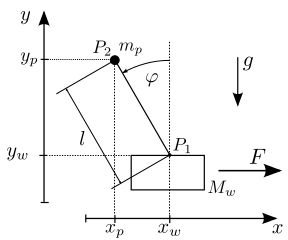
\includegraphics{inv_pendulum.png}

With the \emph{Lagrangian Formalism} the model has the following state
representation where \(u_1 = F\) and
\(x = [x_1, x_2, x_3, x_4] = [x_w, \dot{x}_w, \varphi, \dot{\varphi}]\)
\begin{eqnarray*}
   \dot{x}_1 & = & x_2 \\
   \dot{x}_2 & = & \frac{m_p \sin(x_3)(-l x_4^2 + g \cos x_3)}{M_w l + m_p \sin^2(x_3)} + \frac{\cos(x_3)}{M_w l + m_p l \sin^2(x_3)} u_1 \\
   \dot{x}_3 & = & x_4 \\
   \dot{x}_4 & = & \frac{\sin(x_3)(-m_p l x_4^2 \cos(x_3) + g(M_w + m_p))}{M_w l + m_p \sin^2(x_3)} + \frac{\cos(x_3)}{M_w l + m_p l \sin^2(x_3)} u_1
\end{eqnarray*}
A possibly wanted trajectory is the translation of the cart along the
x-axis (i.e. by \(0.5m\)). In the beginning and end of the process
the cart and pendulum should remain at rest and the pendulum should be
aligned vertically upwards (\(\varphi = 0\)). As a further condition
\(u_1\) should start and end steadily in the rest position
(\(u_1(0) = u_1(T) = 0\)).
The operating time here is \(T = 1 [s]\).


\subsubsection{Source Code}
\label{guide/examples/inv_pendulum_trans:source-code}
\begin{Verbatim}[commandchars=\\\{\}]
\PYG{c}{\PYGZsh{} translation of the inverse pendulum}

\PYG{c}{\PYGZsh{} import trajectory class and necessary dependencies}
\PYG{k+kn}{from} \PYG{n+nn}{pytrajectory} \PYG{k+kn}{import} \PYG{n}{Trajectory}
\PYG{k+kn}{from} \PYG{n+nn}{sympy} \PYG{k+kn}{import} \PYG{n}{sin}\PYG{p}{,} \PYG{n}{cos}
\PYG{k+kn}{import} \PYG{n+nn}{numpy} \PYG{k+kn}{as} \PYG{n+nn}{np}

\PYG{c}{\PYGZsh{} define the function that returns the vectorfield}
\PYG{k}{def} \PYG{n+nf}{f}\PYG{p}{(}\PYG{n}{x}\PYG{p}{,}\PYG{n}{u}\PYG{p}{)}\PYG{p}{:}
    \PYG{n}{x1}\PYG{p}{,} \PYG{n}{x2}\PYG{p}{,} \PYG{n}{x3}\PYG{p}{,} \PYG{n}{x4} \PYG{o}{=} \PYG{n}{x}       \PYG{c}{\PYGZsh{} system state variables}
    \PYG{n}{u1}\PYG{p}{,} \PYG{o}{=} \PYG{n}{u}                  \PYG{c}{\PYGZsh{} input variable}

    \PYG{n}{l} \PYG{o}{=} \PYG{l+m+mf}{0.5}     \PYG{c}{\PYGZsh{} length of the pendulum rod}
    \PYG{n}{g} \PYG{o}{=} \PYG{l+m+mf}{9.81}    \PYG{c}{\PYGZsh{} gravitational acceleration}
    \PYG{n}{M} \PYG{o}{=} \PYG{l+m+mf}{1.0}     \PYG{c}{\PYGZsh{} mass of the cart}
    \PYG{n}{m} \PYG{o}{=} \PYG{l+m+mf}{0.1}     \PYG{c}{\PYGZsh{} mass of the pendulum}

    \PYG{n}{s} \PYG{o}{=} \PYG{n}{sin}\PYG{p}{(}\PYG{n}{x3}\PYG{p}{)}
    \PYG{n}{c} \PYG{o}{=} \PYG{n}{cos}\PYG{p}{(}\PYG{n}{x3}\PYG{p}{)}

    \PYG{n}{ff} \PYG{o}{=} \PYG{n}{np}\PYG{o}{.}\PYG{n}{array}\PYG{p}{(}\PYG{p}{[}                     \PYG{n}{x2}\PYG{p}{,}
                   \PYG{n}{m}\PYG{o}{*}\PYG{n}{s}\PYG{o}{*}\PYG{p}{(}\PYG{o}{\PYGZhy{}}\PYG{n}{l}\PYG{o}{*}\PYG{n}{x4}\PYG{o}{*}\PYG{o}{*}\PYG{l+m+mi}{2}\PYG{o}{+}\PYG{n}{g}\PYG{o}{*}\PYG{n}{c}\PYG{p}{)}\PYG{o}{/}\PYG{p}{(}\PYG{n}{M}\PYG{o}{+}\PYG{n}{m}\PYG{o}{*}\PYG{n}{s}\PYG{o}{*}\PYG{o}{*}\PYG{l+m+mi}{2}\PYG{p}{)}\PYG{o}{+}\PYG{l+m+mi}{1}\PYG{o}{/}\PYG{p}{(}\PYG{n}{M}\PYG{o}{+}\PYG{n}{m}\PYG{o}{*}\PYG{n}{s}\PYG{o}{*}\PYG{o}{*}\PYG{l+m+mi}{2}\PYG{p}{)}\PYG{o}{*}\PYG{n}{u1}\PYG{p}{,}
                                        \PYG{n}{x4}\PYG{p}{,}
            \PYG{n}{s}\PYG{o}{*}\PYG{p}{(}\PYG{o}{\PYGZhy{}}\PYG{n}{m}\PYG{o}{*}\PYG{n}{l}\PYG{o}{*}\PYG{n}{x4}\PYG{o}{*}\PYG{o}{*}\PYG{l+m+mi}{2}\PYG{o}{*}\PYG{n}{c}\PYG{o}{+}\PYG{n}{g}\PYG{o}{*}\PYG{p}{(}\PYG{n}{M}\PYG{o}{+}\PYG{n}{m}\PYG{p}{)}\PYG{p}{)}\PYG{o}{/}\PYG{p}{(}\PYG{n}{M}\PYG{o}{*}\PYG{n}{l}\PYG{o}{+}\PYG{n}{m}\PYG{o}{*}\PYG{n}{l}\PYG{o}{*}\PYG{n}{s}\PYG{o}{*}\PYG{o}{*}\PYG{l+m+mi}{2}\PYG{p}{)}\PYG{o}{+}\PYG{n}{c}\PYG{o}{/}\PYG{p}{(}\PYG{n}{M}\PYG{o}{*}\PYG{n}{l}\PYG{o}{+}\PYG{n}{l}\PYG{o}{*}\PYG{n}{m}\PYG{o}{*}\PYG{n}{s}\PYG{o}{*}\PYG{o}{*}\PYG{l+m+mi}{2}\PYG{p}{)}\PYG{o}{*}\PYG{n}{u1}
                \PYG{p}{]}\PYG{p}{)}
    \PYG{k}{return} \PYG{n}{ff}

\PYG{c}{\PYGZsh{} boundary values at the start (a = 0.0 [s])}
\PYG{n}{xa} \PYG{o}{=} \PYG{p}{[}  \PYG{l+m+mf}{0.0}\PYG{p}{,}
        \PYG{l+m+mf}{0.0}\PYG{p}{,}
        \PYG{l+m+mf}{0.0}\PYG{p}{,}
        \PYG{l+m+mf}{0.0}\PYG{p}{]}

\PYG{c}{\PYGZsh{} boundary values at the end (b = 1.0 [s])}
\PYG{n}{xb} \PYG{o}{=} \PYG{p}{[}  \PYG{l+m+mf}{0.5}\PYG{p}{,}
        \PYG{l+m+mf}{0.0}\PYG{p}{,}
        \PYG{l+m+mf}{0.0}\PYG{p}{,}
        \PYG{l+m+mf}{0.0}\PYG{p}{]}

\PYG{c}{\PYGZsh{} create trajectory object}
\PYG{n}{T} \PYG{o}{=} \PYG{n}{Trajectory}\PYG{p}{(}\PYG{n}{f}\PYG{p}{,} \PYG{n}{a}\PYG{o}{=}\PYG{l+m+mf}{0.0}\PYG{p}{,} \PYG{n}{b}\PYG{o}{=}\PYG{l+m+mf}{1.0}\PYG{p}{,} \PYG{n}{xa}\PYG{o}{=}\PYG{n}{xa}\PYG{p}{,} \PYG{n}{xb}\PYG{o}{=}\PYG{n}{xb}\PYG{p}{)}

\PYG{c}{\PYGZsh{} run iteration}
\PYG{n}{T}\PYG{o}{.}\PYG{n}{startIteration}\PYG{p}{(}\PYG{p}{)}

\PYG{c}{\PYGZsh{} show results}
\PYG{n}{T}\PYG{o}{.}\PYG{n}{plot}\PYG{p}{(}\PYG{p}{)}
\end{Verbatim}


\subsection{Oscillation of the inverted double pendulum}
\label{guide/examples/inv_double_pendulum_swing::doc}\label{guide/examples/inv_double_pendulum_swing:ex-inv-dbl-pend}\label{guide/examples/inv_double_pendulum_swing:oscillation-of-the-inverted-double-pendulum}
In this example we add another pendulum to the cart in the system.

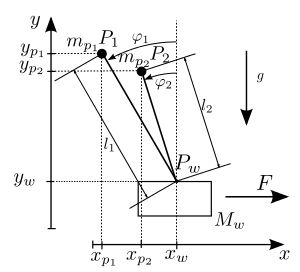
\includegraphics{inv_double_pendulum.png}

The system has the state vector \(x = [x_1, \dot{x}_1,
\varphi_1, \dot{\varphi}_1, \varphi_2, \dot{\varphi}_2]\). A partial
linearization with \(y = x_1\) yields the following system state
representation where \(\tilde{u} = \ddot{y}\).
\begin{eqnarray*}
   \dot{x}_1 & = & x_2 \\
   \dot{x}_2 & = & \tilde{u} \\
   \dot{x}_3 & = & x_4 \\
   \dot{x}_4 & = & \frac{1}{l_1}(g \sin(x_3) + \tilde{u} \cos(x_3)) \\
   \dot{x}_5 & = & x_6 \\
   \dot{x}_6 & = & \frac{1}{l_2}(g \sin(x_5) + \tilde{u} \cos(x_5))
\end{eqnarray*}
Here a trajectory should be planned that transfers the system between
the following two positions of rest. At the beginning both pendulums
should be directed downwards (\(\varphi_1 = \varphi_2 = \pi\)).
After a operating time of \(T = 2 [s]\) the cart should be at the
same position again and the pendulums should be at rest with
\(\varphi_1 = \varphi_2 = 0\).
\begin{equation*}
   x(0) = \begin{bmatrix} 0 \\ 0 \\ \pi \\ 0 \\ \pi \\ 0 \end{bmatrix}
   \rightarrow
   x(T) = \begin{bmatrix} 0 \\ 0 \\ 0 \\ 0 \\ 0 \\ 0 \end{bmatrix}
\end{equation*}

\subsubsection{Source Code}
\label{guide/examples/inv_double_pendulum_swing:source-code}
\begin{Verbatim}[commandchars=\\\{\}]
\PYG{c}{\PYGZsh{} oscillation of the inverted double pendulum with partial linearization}

\PYG{c}{\PYGZsh{} import trajectory class and necessary dependencies}
\PYG{k+kn}{from} \PYG{n+nn}{pytrajectory.trajectory} \PYG{k+kn}{import} \PYG{n}{Trajectory}
\PYG{k+kn}{from} \PYG{n+nn}{sympy} \PYG{k+kn}{import} \PYG{n}{cos}\PYG{p}{,} \PYG{n}{sin}
\PYG{k+kn}{import} \PYG{n+nn}{numpy} \PYG{k+kn}{as} \PYG{n+nn}{np}
\PYG{k+kn}{from} \PYG{n+nn}{numpy} \PYG{k+kn}{import} \PYG{n}{pi}

\PYG{c}{\PYGZsh{} define the function that returns the vectorfield}
\PYG{k}{def} \PYG{n+nf}{f}\PYG{p}{(}\PYG{n}{x}\PYG{p}{,}\PYG{n}{u}\PYG{p}{)}\PYG{p}{:}
	\PYG{n}{x1}\PYG{p}{,} \PYG{n}{x2}\PYG{p}{,} \PYG{n}{x3}\PYG{p}{,} \PYG{n}{x4}\PYG{p}{,} \PYG{n}{x5}\PYG{p}{,} \PYG{n}{x6} \PYG{o}{=} \PYG{n}{x}  \PYG{c}{\PYGZsh{} system variables}
	\PYG{n}{u}\PYG{p}{,} \PYG{o}{=} \PYG{n}{u}                      \PYG{c}{\PYGZsh{} input variable}
    
    \PYG{c}{\PYGZsh{} length of the pendulums}
	\PYG{n}{l1} \PYG{o}{=} \PYG{l+m+mf}{0.7}
	\PYG{n}{l2} \PYG{o}{=} \PYG{l+m+mf}{0.5}
    
	\PYG{n}{g} \PYG{o}{=} \PYG{l+m+mf}{9.81}    \PYG{c}{\PYGZsh{} gravitational acceleration}
    
	\PYG{n}{ff} \PYG{o}{=} \PYG{n}{np}\PYG{o}{.}\PYG{n}{array}\PYG{p}{(}\PYG{p}{[}         \PYG{n}{x2}\PYG{p}{,}
                            \PYG{n}{u}\PYG{p}{,}
                            \PYG{n}{x4}\PYG{p}{,}
                \PYG{p}{(}\PYG{l+m+mi}{1}\PYG{o}{/}\PYG{n}{l1}\PYG{p}{)}\PYG{o}{*}\PYG{p}{(}\PYG{n}{g}\PYG{o}{*}\PYG{n}{sin}\PYG{p}{(}\PYG{n}{x3}\PYG{p}{)}\PYG{o}{+}\PYG{n}{u}\PYG{o}{*}\PYG{n}{cos}\PYG{p}{(}\PYG{n}{x3}\PYG{p}{)}\PYG{p}{)}\PYG{p}{,}
                            \PYG{n}{x6}\PYG{p}{,}
                \PYG{p}{(}\PYG{l+m+mi}{1}\PYG{o}{/}\PYG{n}{l2}\PYG{p}{)}\PYG{o}{*}\PYG{p}{(}\PYG{n}{g}\PYG{o}{*}\PYG{n}{sin}\PYG{p}{(}\PYG{n}{x5}\PYG{p}{)}\PYG{o}{+}\PYG{n}{u}\PYG{o}{*}\PYG{n}{cos}\PYG{p}{(}\PYG{n}{x5}\PYG{p}{)}\PYG{p}{)}
                    \PYG{p}{]}\PYG{p}{)}
    
	\PYG{k}{return} \PYG{n}{ff}

\PYG{c}{\PYGZsh{} system state boundary values for a = 0.0 [s] and b = 2.0 [s]}
\PYG{n}{xa} \PYG{o}{=} \PYG{p}{[}\PYG{l+m+mf}{0.0}\PYG{p}{,} \PYG{l+m+mf}{0.0}\PYG{p}{,}  \PYG{n}{pi}\PYG{p}{,} \PYG{l+m+mf}{0.0}\PYG{p}{,}  \PYG{n}{pi}\PYG{p}{,} \PYG{l+m+mf}{0.0}\PYG{p}{]}
\PYG{n}{xb} \PYG{o}{=} \PYG{p}{[}\PYG{l+m+mf}{0.0}\PYG{p}{,} \PYG{l+m+mf}{0.0}\PYG{p}{,} \PYG{l+m+mf}{0.0}\PYG{p}{,} \PYG{l+m+mf}{0.0}\PYG{p}{,} \PYG{l+m+mf}{0.0}\PYG{p}{,} \PYG{l+m+mf}{0.0}\PYG{p}{]}

\PYG{c}{\PYGZsh{} boundary values for the input}
\PYG{n}{g}\PYG{o}{=} \PYG{p}{[}\PYG{l+m+mf}{0.0}\PYG{p}{,} \PYG{l+m+mf}{0.0}\PYG{p}{]}

\PYG{c}{\PYGZsh{} create trajectory object}
\PYG{n}{T} \PYG{o}{=} \PYG{n}{Trajectory}\PYG{p}{(}\PYG{n}{f}\PYG{p}{,} \PYG{n}{a}\PYG{o}{=}\PYG{l+m+mf}{0.0}\PYG{p}{,} \PYG{n}{b}\PYG{o}{=}\PYG{l+m+mf}{2.0}\PYG{p}{,} \PYG{n}{xa}\PYG{o}{=}\PYG{n}{xa}\PYG{p}{,} \PYG{n}{xb}\PYG{o}{=}\PYG{n}{xb}\PYG{p}{,} \PYG{n}{g}\PYG{o}{=}\PYG{n}{g}\PYG{p}{)}

\PYG{c}{\PYGZsh{} alter some method parameters to increase performance}
\PYG{n}{T}\PYG{o}{.}\PYG{n}{setParam}\PYG{p}{(}\PYG{l+s}{\PYGZsq{}}\PYG{l+s}{su}\PYG{l+s}{\PYGZsq{}}\PYG{p}{,} \PYG{l+m+mi}{10}\PYG{p}{)}
\PYG{n}{T}\PYG{o}{.}\PYG{n}{setParam}\PYG{p}{(}\PYG{l+s}{\PYGZsq{}}\PYG{l+s}{eps}\PYG{l+s}{\PYGZsq{}}\PYG{p}{,} \PYG{l+m+mf}{8e\PYGZhy{}2}\PYG{p}{)}

\PYG{c}{\PYGZsh{} run iteration}
\PYG{n}{T}\PYG{o}{.}\PYG{n}{startIteration}\PYG{p}{(}\PYG{p}{)}

\PYG{c}{\PYGZsh{} show results}
\PYG{n}{T}\PYG{o}{.}\PYG{n}{plot}\PYG{p}{(}\PYG{p}{)}
\end{Verbatim}


\subsection{Aircraft}
\label{guide/examples/aircraft:ex-aircraft}\label{guide/examples/aircraft:aircraft}\label{guide/examples/aircraft::doc}
In this section we consider the model of a unmanned vertical take-off
aircraft. The aircraft has two permanently mounted thrusters on the
wings which can apply the thrust forces \(F_1\) and \(F_2\)
independently of each other. The two engines are inclined by an angle
\(\alpha\) with respect to the aircraft-fixed axis \(\eta_2\)
and engage in the points \(P_1 = (l, h)\) and \(P_2 = (-l,-h)\).
The coordinates of the center of mass \(M\) of the aircraft in the
inertial system are denoted by \(z_1\) and \(z_2\). At the same
time, the point is the origin of the plane coordinate system. The
aircraft axes are rotated by the angle \(\theta\) with respect to
the \(z_2\)-axis.

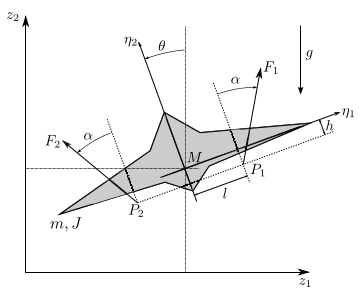
\includegraphics{aircraft.png}

Through the establishment of the momentum balances for the model one
obtains the equations
\begin{eqnarray*}
   m \ddot{z}_1 & = & - \sin(\theta)(F_1 + F_2)\cos(\alpha) + \cos(\theta)(F_1 - F_2)\sin(\alpha) \\
   m \ddot{z}_2 & = & \cos(\theta)(F_1 + F_2)\sin(\alpha) + \sin(\theta)(F_1 - F_2)\cos(\alpha) - mg \\
   J \ddot{\theta} & = & (F_1 - F_2)(l \cos(\alpha) + h \sin(\alpha))
\end{eqnarray*}
With the state vector \(x = [z_1, \dot{z}_1, z_2, \dot{z}_2, \theta, \dot{\theta}]^T\)
and \(u = [u_1, u_2]^T = [F_1, F_2]^T\) the state space
representation of the system is as follows.
\begin{eqnarray*}
   \dot{x}_1 & = & x_2 \\
   \dot{x}_2 & = & \frac{1}{m}(-\sin(x_5)(u_1 + u_2)\cos(\alpha) + \cos(x_5)(u_1 - u_2)\sin(\alpha)) \\
   \dot{x}_3 & = & x_4 \\
   \dot{x}_2 & = & \frac{1}{m}(\cos(x_5)(u_1 + u_2)\cos(\alpha) + \sin(x_5)(u_1 - u_2)\sin(\alpha)) - g  \\
   \dot{x}_5 & = & x_6 \\
   \dot{x}_6 & = & \frac{1}{J}(l \cos(\alpha) + h \sin(\alpha))
\end{eqnarray*}
For the aircraft, a trajectory should be planned that translates the
horizontally aligned flying object from a rest position (hovering) along
the \(z_1\) and \(z_2\) axis back into a hovering position.
The hovering is to be realized on the boundary conditions of the input.
Therefor the derivatives of the state variables should satisfy the
following conditions.
$ \dot{z}_1 = \ddot{z}_1 = \dot{z}_2 = \ddot{z_2} = \dot{\theta} = \ddot{\theta} = 0 $
For the horizontal position applies \(\theta = 0\). These demands
yield the boundary conditions for the inputs.
$ F_1(0) = F_1(T) = F_2(0) = F_2(T) = \frac{mg}{2 \cos(\alpha)} $

\subsubsection{Source Code}
\label{guide/examples/aircraft:source-code}
\begin{Verbatim}[commandchars=\\\{\}]
\PYG{c}{\PYGZsh{} vertical take\PYGZhy{}off aircraft}

\PYG{c}{\PYGZsh{} import trajectory class and necessary dependencies}
\PYG{k+kn}{from} \PYG{n+nn}{pytrajectory} \PYG{k+kn}{import} \PYG{n}{Trajectory}
\PYG{k+kn}{from} \PYG{n+nn}{sympy} \PYG{k+kn}{import} \PYG{n}{sin}\PYG{p}{,} \PYG{n}{cos}
\PYG{k+kn}{import} \PYG{n+nn}{numpy} \PYG{k+kn}{as} \PYG{n+nn}{np}
\PYG{k+kn}{from} \PYG{n+nn}{numpy} \PYG{k+kn}{import} \PYG{n}{pi}

\PYG{c}{\PYGZsh{} define the function that returns the vectorfield}
\PYG{k}{def} \PYG{n+nf}{f}\PYG{p}{(}\PYG{n}{x}\PYG{p}{,}\PYG{n}{u}\PYG{p}{)}\PYG{p}{:}
    \PYG{n}{x1}\PYG{p}{,} \PYG{n}{x2}\PYG{p}{,} \PYG{n}{x3}\PYG{p}{,} \PYG{n}{x4}\PYG{p}{,} \PYG{n}{x5}\PYG{p}{,} \PYG{n}{x6} \PYG{o}{=} \PYG{n}{x}  \PYG{c}{\PYGZsh{} system state variables}
    \PYG{n}{u1}\PYG{p}{,} \PYG{n}{u2} \PYG{o}{=} \PYG{n}{u}                  \PYG{c}{\PYGZsh{} input variables}
    
    \PYG{c}{\PYGZsh{} coordinates for the points in which the engines engage [m]}
    \PYG{n}{l} \PYG{o}{=} \PYG{l+m+mf}{1.0}
    \PYG{n}{h} \PYG{o}{=} \PYG{l+m+mf}{0.1}

    \PYG{n}{g} \PYG{o}{=} \PYG{l+m+mf}{9.81}    \PYG{c}{\PYGZsh{} graviational acceleration [m/s\PYGZca{}2]}
    \PYG{n}{M} \PYG{o}{=} \PYG{l+m+mf}{50.0}    \PYG{c}{\PYGZsh{} mass of the aircraft [kg]}
    \PYG{n}{J} \PYG{o}{=} \PYG{l+m+mf}{25.0}    \PYG{c}{\PYGZsh{} moment of inertia about M [kg*m\PYGZca{}2]}

    \PYG{n}{alpha} \PYG{o}{=} \PYG{l+m+mi}{5}\PYG{o}{/}\PYG{l+m+mf}{360.0}\PYG{o}{*}\PYG{l+m+mi}{2}\PYG{o}{*}\PYG{n}{pi}    \PYG{c}{\PYGZsh{} deflection of the engines}

    \PYG{n}{sa} \PYG{o}{=} \PYG{n}{sin}\PYG{p}{(}\PYG{n}{alpha}\PYG{p}{)}
    \PYG{n}{ca} \PYG{o}{=} \PYG{n}{cos}\PYG{p}{(}\PYG{n}{alpha}\PYG{p}{)}

    \PYG{n}{s} \PYG{o}{=} \PYG{n}{sin}\PYG{p}{(}\PYG{n}{x5}\PYG{p}{)}
    \PYG{n}{c} \PYG{o}{=} \PYG{n}{cos}\PYG{p}{(}\PYG{n}{x5}\PYG{p}{)}
    
    \PYG{n}{ff} \PYG{o}{=} \PYG{n}{np}\PYG{o}{.}\PYG{n}{array}\PYG{p}{(}\PYG{p}{[}             \PYG{n}{x2}\PYG{p}{,}
                    \PYG{o}{\PYGZhy{}}\PYG{n}{s}\PYG{o}{/}\PYG{n}{M}\PYG{o}{*}\PYG{p}{(}\PYG{n}{u1}\PYG{o}{+}\PYG{n}{u2}\PYG{p}{)} \PYG{o}{+} \PYG{n}{c}\PYG{o}{/}\PYG{n}{M}\PYG{o}{*}\PYG{p}{(}\PYG{n}{u1}\PYG{o}{\PYGZhy{}}\PYG{n}{u2}\PYG{p}{)}\PYG{o}{*}\PYG{n}{sa}\PYG{p}{,}
                                \PYG{n}{x4}\PYG{p}{,}
                    \PYG{o}{\PYGZhy{}}\PYG{n}{g}\PYG{o}{+}\PYG{n}{c}\PYG{o}{/}\PYG{n}{M}\PYG{o}{*}\PYG{p}{(}\PYG{n}{u1}\PYG{o}{+}\PYG{n}{u2}\PYG{p}{)} \PYG{o}{+}\PYG{n}{s}\PYG{o}{/}\PYG{n}{M}\PYG{o}{*}\PYG{p}{(}\PYG{n}{u1}\PYG{o}{\PYGZhy{}}\PYG{n}{u2}\PYG{p}{)}\PYG{o}{*}\PYG{n}{sa} \PYG{p}{,}
                                \PYG{n}{x6}\PYG{p}{,}
                    \PYG{l+m+mi}{1}\PYG{o}{/}\PYG{n}{J}\PYG{o}{*}\PYG{p}{(}\PYG{n}{u1}\PYG{o}{\PYGZhy{}}\PYG{n}{u2}\PYG{p}{)}\PYG{o}{*}\PYG{p}{(}\PYG{n}{l}\PYG{o}{*}\PYG{n}{ca}\PYG{o}{+}\PYG{n}{h}\PYG{o}{*}\PYG{n}{sa}\PYG{p}{)}\PYG{p}{]}\PYG{p}{)}
    
    \PYG{k}{return} \PYG{n}{ff} 

\PYG{c}{\PYGZsh{} system state boundary values for a = 0.0 [s] and b = 3.0 [s]}
\PYG{n}{xa} \PYG{o}{=} \PYG{p}{[} \PYG{l+m+mf}{0.0}\PYG{p}{,} \PYG{l+m+mf}{0.0}\PYG{p}{,} \PYG{l+m+mf}{0.0}\PYG{p}{,} \PYG{l+m+mf}{0.0}\PYG{p}{,} \PYG{l+m+mf}{0.0}\PYG{p}{,} \PYG{l+m+mf}{0.0}\PYG{p}{]}
\PYG{n}{xb} \PYG{o}{=} \PYG{p}{[}\PYG{l+m+mf}{10.0}\PYG{p}{,} \PYG{l+m+mf}{0.0}\PYG{p}{,} \PYG{l+m+mf}{5.0}\PYG{p}{,} \PYG{l+m+mf}{0.0}\PYG{p}{,} \PYG{l+m+mf}{0.0}\PYG{p}{,} \PYG{l+m+mf}{0.0}\PYG{p}{]}

\PYG{c}{\PYGZsh{} boundary values for the inputs}
\PYG{n}{g} \PYG{o}{=} \PYG{p}{[}\PYG{l+m+mf}{0.5}\PYG{o}{*}\PYG{l+m+mf}{9.81}\PYG{o}{*}\PYG{l+m+mf}{50.0}\PYG{o}{/}\PYG{p}{(}\PYG{n}{cos}\PYG{p}{(}\PYG{l+m+mi}{5}\PYG{o}{/}\PYG{l+m+mf}{360.0}\PYG{o}{*}\PYG{l+m+mi}{2}\PYG{o}{*}\PYG{n}{pi}\PYG{p}{)}\PYG{p}{)}\PYG{p}{,}
     \PYG{l+m+mf}{0.5}\PYG{o}{*}\PYG{l+m+mf}{9.81}\PYG{o}{*}\PYG{l+m+mf}{50.0}\PYG{o}{/}\PYG{p}{(}\PYG{n}{cos}\PYG{p}{(}\PYG{l+m+mi}{5}\PYG{o}{/}\PYG{l+m+mf}{360.0}\PYG{o}{*}\PYG{l+m+mi}{2}\PYG{o}{*}\PYG{n}{pi}\PYG{p}{)}\PYG{p}{)}\PYG{p}{]}

\PYG{c}{\PYGZsh{} create trajectory object}
\PYG{n}{T} \PYG{o}{=} \PYG{n}{Trajectory}\PYG{p}{(}\PYG{n}{f}\PYG{p}{,} \PYG{n}{a}\PYG{o}{=}\PYG{l+m+mf}{0.0}\PYG{p}{,} \PYG{n}{b}\PYG{o}{=}\PYG{l+m+mf}{3.0}\PYG{p}{,} \PYG{n}{xa}\PYG{o}{=}\PYG{n}{xa}\PYG{p}{,} \PYG{n}{xb}\PYG{o}{=}\PYG{n}{xb}\PYG{p}{,} \PYG{n}{g}\PYG{o}{=}\PYG{n}{g}\PYG{p}{)}

\PYG{c}{\PYGZsh{} don\PYGZsq{}t take advantage of the system structure (integrator chains)}
\PYG{c}{\PYGZsh{} (this will result in a faster solution here)}
\PYG{n}{T}\PYG{o}{.}\PYG{n}{setParam}\PYG{p}{(}\PYG{l+s}{\PYGZsq{}}\PYG{l+s}{use\PYGZus{}chains}\PYG{l+s}{\PYGZsq{}}\PYG{p}{,} \PYG{n+nb+bp}{False}\PYG{p}{)}

\PYG{c}{\PYGZsh{} also alter some other method parameters to increase performance}
\PYG{n}{T}\PYG{o}{.}\PYG{n}{setParam}\PYG{p}{(}\PYG{l+s}{\PYGZsq{}}\PYG{l+s}{kx}\PYG{l+s}{\PYGZsq{}}\PYG{p}{,} \PYG{l+m+mi}{5}\PYG{p}{)}

\PYG{c}{\PYGZsh{} run iteration}
\PYG{n}{T}\PYG{o}{.}\PYG{n}{startIteration}\PYG{p}{(}\PYG{p}{)}

\PYG{c}{\PYGZsh{} show results}
\PYG{n}{T}\PYG{o}{.}\PYG{n}{plot}\PYG{p}{(}\PYG{p}{)}
\end{Verbatim}


\subsection{Underactuated Manipulator}
\label{guide/examples/uact_manipulator:ex-unact-mani}\label{guide/examples/uact_manipulator::doc}\label{guide/examples/uact_manipulator:underactuated-manipulator}
In this section, the model of an underactuated manipulator is treated.
The system consists of two bars with the mass \(M_1\) and
\(M_2\) which are connected to each other via the joint \(G_2\).
The angle between them is designated by \(\theta_2\). The joint
\(G_1\) connects the first rod with the inertial system, the angle
to the \(x\)-axis is labeled \(\theta_1\).
In the joint \(G_1\) the actuating torque \(Q\) is applied. The
bars have the moments of inertia \(I_1\) and \(I_2\). The
distances between the centers of mass to the joints are \(r_1\) and
\(r_2\).

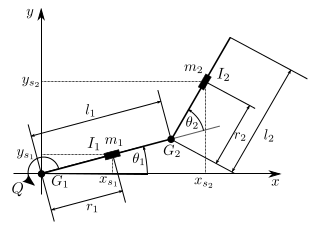
\includegraphics{uact_manipulator.png}

The modeling was taken from the thesis of Carsten Knoll
(April, 2009) where in addition the inertia parameter \(\eta\) was
introduced.
\begin{equation*}
   \eta = \frac{m_2 l_1 r_2}{I_2 + m_2 r_2^2}
\end{equation*}
For the example shown here, strong inertia coupling was assumed with
\(\eta = 0.9\). By partial linearization to the output \(y =
\theta_1\) one obtains the state representation with the states
\(x = [\theta_1, \dot{\theta}_1, \theta_2, \dot{\theta}_2]^T\) and
the new input \(\tilde{u} = \ddot{\theta}_1\).
\begin{eqnarray*}
   \dot{x}_1 & = & x_2 \\
   \dot{x}_2 & = & \tilde{u} \\
   \dot{x}_3 & = & x_4 \\
   \dot{x}_4 & = & -\eta x_2^2  \sin(x_3) - (1 + \eta \cos(x_3))\tilde{u}
\end{eqnarray*}
For the system, a trajectory is to be determined for the transfer
between two equilibrium positions within an operating time of
\(T = 1.8 [s]\).
\begin{equation*}
   x(0) = \begin{bmatrix} 0 \\ 0 \\ 0.4 \pi \\ 0 \end{bmatrix}
   \rightarrow
   x(T) = \begin{bmatrix} 0.2 \pi \\ 0 \\ 0.2 \pi \\ 0 \end{bmatrix}
\end{equation*}
The trajectory of the inputs should be without cracks in the transition
to the equilibrium positions (\(\tilde{u}(0) = \tilde{u}(T) = 0\)).


\subsubsection{Source Code}
\label{guide/examples/uact_manipulator:source-code}
\begin{Verbatim}[commandchars=\\\{\}]
\PYG{c}{\PYGZsh{} underactuated manipulator}

\PYG{c}{\PYGZsh{} import trajectory class and necessary dependencies}
\PYG{k+kn}{from} \PYG{n+nn}{pytrajectory.trajectory} \PYG{k+kn}{import} \PYG{n}{Trajectory}
\PYG{k+kn}{import} \PYG{n+nn}{numpy} \PYG{k+kn}{as} \PYG{n+nn}{np}
\PYG{k+kn}{from} \PYG{n+nn}{sympy} \PYG{k+kn}{import} \PYG{n}{cos}\PYG{p}{,} \PYG{n}{sin}
\PYG{k+kn}{from} \PYG{n+nn}{numpy} \PYG{k+kn}{import} \PYG{n}{pi}

\PYG{c}{\PYGZsh{} define the function that returns the vectorfield}
\PYG{k}{def} \PYG{n+nf}{f}\PYG{p}{(}\PYG{n}{x}\PYG{p}{,}\PYG{n}{u}\PYG{p}{)}\PYG{p}{:}
    \PYG{n}{x1}\PYG{p}{,} \PYG{n}{x2}\PYG{p}{,} \PYG{n}{x3}\PYG{p}{,} \PYG{n}{x4}  \PYG{o}{=} \PYG{n}{x}     \PYG{c}{\PYGZsh{} state variables}
    \PYG{n}{u1}\PYG{p}{,} \PYG{o}{=} \PYG{n}{u}                 \PYG{c}{\PYGZsh{} input variable}
    
    \PYG{n}{e} \PYG{o}{=} \PYG{l+m+mf}{0.9}     \PYG{c}{\PYGZsh{} inertia coupling}
    
    \PYG{n}{s} \PYG{o}{=} \PYG{n}{sin}\PYG{p}{(}\PYG{n}{x3}\PYG{p}{)}
    \PYG{n}{c} \PYG{o}{=} \PYG{n}{cos}\PYG{p}{(}\PYG{n}{x3}\PYG{p}{)}
    
    \PYG{n}{ff} \PYG{o}{=} \PYG{n}{np}\PYG{o}{.}\PYG{n}{array}\PYG{p}{(}\PYG{p}{[}         \PYG{n}{x2}\PYG{p}{,}
                            \PYG{n}{u1}\PYG{p}{,}
                            \PYG{n}{x4}\PYG{p}{,}
                    \PYG{o}{\PYGZhy{}}\PYG{n}{e}\PYG{o}{*}\PYG{n}{x2}\PYG{o}{*}\PYG{o}{*}\PYG{l+m+mi}{2}\PYG{o}{*}\PYG{n}{s}\PYG{o}{\PYGZhy{}}\PYG{p}{(}\PYG{l+m+mi}{1}\PYG{o}{+}\PYG{n}{e}\PYG{o}{*}\PYG{n}{c}\PYG{p}{)}\PYG{o}{*}\PYG{n}{u1}
                    \PYG{p}{]}\PYG{p}{)}
    
    \PYG{k}{return} \PYG{n}{ff}

\PYG{c}{\PYGZsh{} system state boundary values for a = 0.0 [s] and b = 1.8 [s]}
\PYG{n}{xa} \PYG{o}{=} \PYG{p}{[}  \PYG{l+m+mf}{0.0}\PYG{p}{,}
        \PYG{l+m+mf}{0.0}\PYG{p}{,}
        \PYG{l+m+mf}{0.4}\PYG{o}{*}\PYG{n}{pi}\PYG{p}{,}
        \PYG{l+m+mf}{0.0}\PYG{p}{]}

\PYG{n}{xb} \PYG{o}{=} \PYG{p}{[}  \PYG{l+m+mf}{0.2}\PYG{o}{*}\PYG{n}{pi}\PYG{p}{,}
        \PYG{l+m+mf}{0.0}\PYG{p}{,}
        \PYG{l+m+mf}{0.2}\PYG{o}{*}\PYG{n}{pi}\PYG{p}{,}
        \PYG{l+m+mf}{0.0}\PYG{p}{]}

\PYG{c}{\PYGZsh{} boundary values for the inputs}
\PYG{n}{g} \PYG{o}{=} \PYG{p}{[}\PYG{l+m+mf}{0.0}\PYG{p}{,} \PYG{l+m+mf}{0.0}\PYG{p}{]}

\PYG{c}{\PYGZsh{} create trajectory object}
\PYG{n}{T} \PYG{o}{=} \PYG{n}{Trajectory}\PYG{p}{(}\PYG{n}{f}\PYG{p}{,} \PYG{n}{a}\PYG{o}{=}\PYG{l+m+mf}{0.0}\PYG{p}{,} \PYG{n}{b}\PYG{o}{=}\PYG{l+m+mf}{1.8}\PYG{p}{,} \PYG{n}{xa}\PYG{o}{=}\PYG{n}{xa}\PYG{p}{,} \PYG{n}{xb}\PYG{o}{=}\PYG{n}{xb}\PYG{p}{,} \PYG{n}{g}\PYG{o}{=}\PYG{n}{g}\PYG{p}{)}

\PYG{c}{\PYGZsh{} also alter some method parameters to increase performance}
\PYG{n}{T}\PYG{o}{.}\PYG{n}{setParam}\PYG{p}{(}\PYG{l+s}{\PYGZsq{}}\PYG{l+s}{su}\PYG{l+s}{\PYGZsq{}}\PYG{p}{,} \PYG{l+m+mi}{20}\PYG{p}{)}
\PYG{n}{T}\PYG{o}{.}\PYG{n}{setParam}\PYG{p}{(}\PYG{l+s}{\PYGZsq{}}\PYG{l+s}{kx}\PYG{l+s}{\PYGZsq{}}\PYG{p}{,} \PYG{l+m+mi}{3}\PYG{p}{)}

\PYG{c}{\PYGZsh{} run iteration}
\PYG{n}{T}\PYG{o}{.}\PYG{n}{startIteration}\PYG{p}{(}\PYG{p}{)}

\PYG{c}{\PYGZsh{} show results}
\PYG{n}{T}\PYG{o}{.}\PYG{n}{plot}\PYG{p}{(}\PYG{p}{)}
\end{Verbatim}


\subsection{Acrobot}
\label{guide/examples/acrobot:ex-acrobot}\label{guide/examples/acrobot::doc}\label{guide/examples/acrobot:acrobot}
One further interesting example is that of the acrobot. The model can be
regarded as a simplified gymnast hanging on a horizontal bar with both hands.
The movements of the entire system is to be controlled only by movement of the hip.
The body of the gymnast is represented by two rods which are jointed in the joint
\(G_2\). The first rod is movably connected at joint \(G_1\) with the inertial
system, which corresponds to the encompassing of the stretching rod with the hands.

For the model, two equal-length rods with a length \(l_1 = l_2 = l\) are assumed
with a homogeneous distribution of mass \(m_1 = m_2 = m\) over the entire rod length.
This does not correspond to the proportions of a man, also no restrictions were placed
on the mobility of the hip joint.

The following figure shows the schematic representation of the model.

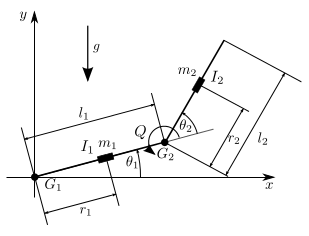
\includegraphics{acrobot.png}

Using the previously assumed model parameters and the write abbreviations
\begin{eqnarray*}
   I      & = & \frac{1}{3}m l^2 \\
   d_{11} & = & \frac{m l^2}{4} + m(l^2 + \frac{l^2}{4} + l^2 \cos(\theta_2)) + 2I \\
   h_1    & = & - \frac{m l^2}{2} \sin(\theta_2) (\dot{\theta}_2 (\dot{\theta}_2 + 2\dot{\theta}_1)) \\
   d_{12} & = & m (\frac{l^2}{4} + \frac{l^2}{2} \cos(\theta_1)) + I \\
   \varphi_1 & = & \frac{3}{2}m l g \cos(\theta_1) + \frac{1}{2}m l g \cos(\theta_1 + \theta_2)
 \end{eqnarray*}
as well as the state vector \(x = [\theta_2, \dot{\theta}_2, \theta_1, \dot{\theta}_1]\) one obtains
the following state representation with the virtual input \(u = \ddot{\theta}_2\)
\begin{eqnarray*}
   \dot{x}_1 & = & x_2 \\
   \dot{x}_2 & = & u \\
   \dot{x}_3 & = & x_4 \\
   \dot{x}_4 & = & -d_{11}^{-1} (h_1 + \varphi_1 + d_{12}u)
\end{eqnarray*}
Now, the trajectory of the manipulated variable for an oscillation of the gymnast should be determined.
The starting point of the exercise are the two downward hanging rods. These are to be transferred into another
rest position in which the two bars show vertically upward within an operating time of \(T = 2 [s]\).
At the beginning and end of the process, the input variable is to merge continuously into the rest
position \(u(0) = u(T) = 0\).

The initial and final states thus are
\begin{equation*}
   x(0) = \begin{bmatrix} 0 \\ 0 \\ \frac{3}{2} \pi \\ 0 \end{bmatrix}
   \rightarrow
   x(T) = \begin{bmatrix} 0 \\ 0 \\ \frac{1}{2} \pi \\ 0 \end{bmatrix}
\end{equation*}

\subsubsection{Source Code}
\label{guide/examples/acrobot:source-code}
\begin{Verbatim}[commandchars=\\\{\}]
\PYG{c}{\PYGZsh{} acrobot}

\PYG{c}{\PYGZsh{} import trajectory class and necessary dependencies}
\PYG{k+kn}{from} \PYG{n+nn}{pytrajectory.trajectory} \PYG{k+kn}{import} \PYG{n}{Trajectory}
\PYG{k+kn}{import} \PYG{n+nn}{numpy} \PYG{k+kn}{as} \PYG{n+nn}{np}
\PYG{k+kn}{from} \PYG{n+nn}{sympy} \PYG{k+kn}{import} \PYG{n}{cos}\PYG{p}{,} \PYG{n}{sin}
\PYG{k+kn}{from} \PYG{n+nn}{numpy} \PYG{k+kn}{import} \PYG{n}{pi}

\PYG{c}{\PYGZsh{} define the function that returns the vectorfield}
\PYG{k}{def} \PYG{n+nf}{f}\PYG{p}{(}\PYG{n}{x}\PYG{p}{,}\PYG{n}{u}\PYG{p}{)}\PYG{p}{:}
    \PYG{n}{x1}\PYG{p}{,} \PYG{n}{x2}\PYG{p}{,} \PYG{n}{x3}\PYG{p}{,} \PYG{n}{x4} \PYG{o}{=} \PYG{n}{x}
    \PYG{n}{u1}\PYG{p}{,} \PYG{o}{=} \PYG{n}{u}
    
    \PYG{n}{m} \PYG{o}{=} \PYG{l+m+mf}{1.0}             \PYG{c}{\PYGZsh{} masses of the rods [m1 = m2 = m]}
    \PYG{n}{l} \PYG{o}{=} \PYG{l+m+mf}{0.5}             \PYG{c}{\PYGZsh{} lengths of the rods [l1 = l2 = l]}
    
    \PYG{n}{I} \PYG{o}{=} \PYG{l+m+mi}{1}\PYG{o}{/}\PYG{l+m+mf}{3.0}\PYG{o}{*}\PYG{n}{m}\PYG{o}{*}\PYG{n}{l}\PYG{o}{*}\PYG{o}{*}\PYG{l+m+mi}{2}    \PYG{c}{\PYGZsh{} moments of inertia [I1 = I2 = I]}
    \PYG{n}{g} \PYG{o}{=} \PYG{l+m+mf}{9.81}            \PYG{c}{\PYGZsh{} gravitational acceleration}
    
    \PYG{n}{lc} \PYG{o}{=} \PYG{n}{l}\PYG{o}{/}\PYG{l+m+mf}{2.0}
    
    \PYG{n}{d11} \PYG{o}{=} \PYG{n}{m}\PYG{o}{*}\PYG{n}{lc}\PYG{o}{*}\PYG{o}{*}\PYG{l+m+mi}{2}\PYG{o}{+}\PYG{n}{m}\PYG{o}{*}\PYG{p}{(}\PYG{n}{l}\PYG{o}{*}\PYG{o}{*}\PYG{l+m+mi}{2}\PYG{o}{+}\PYG{n}{lc}\PYG{o}{*}\PYG{o}{*}\PYG{l+m+mi}{2}\PYG{o}{+}\PYG{l+m+mi}{2}\PYG{o}{*}\PYG{n}{l}\PYG{o}{*}\PYG{n}{lc}\PYG{o}{*}\PYG{n}{cos}\PYG{p}{(}\PYG{n}{x1}\PYG{p}{)}\PYG{p}{)}\PYG{o}{+}\PYG{l+m+mi}{2}\PYG{o}{*}\PYG{n}{I}
    \PYG{n}{h1} \PYG{o}{=} \PYG{o}{\PYGZhy{}}\PYG{n}{m}\PYG{o}{*}\PYG{n}{l}\PYG{o}{*}\PYG{n}{lc}\PYG{o}{*}\PYG{n}{sin}\PYG{p}{(}\PYG{n}{x1}\PYG{p}{)}\PYG{o}{*}\PYG{p}{(}\PYG{n}{x2}\PYG{o}{*}\PYG{p}{(}\PYG{n}{x2}\PYG{o}{+}\PYG{l+m+mi}{2}\PYG{o}{*}\PYG{n}{x4}\PYG{p}{)}\PYG{p}{)}
    \PYG{n}{d12} \PYG{o}{=} \PYG{n}{m}\PYG{o}{*}\PYG{p}{(}\PYG{n}{lc}\PYG{o}{*}\PYG{o}{*}\PYG{l+m+mi}{2}\PYG{o}{+}\PYG{n}{l}\PYG{o}{*}\PYG{n}{lc}\PYG{o}{*}\PYG{n}{cos}\PYG{p}{(}\PYG{n}{x1}\PYG{p}{)}\PYG{p}{)}\PYG{o}{+}\PYG{n}{I}
    \PYG{n}{phi1} \PYG{o}{=} \PYG{p}{(}\PYG{n}{m}\PYG{o}{*}\PYG{n}{lc}\PYG{o}{+}\PYG{n}{m}\PYG{o}{*}\PYG{n}{l}\PYG{p}{)}\PYG{o}{*}\PYG{n}{g}\PYG{o}{*}\PYG{n}{cos}\PYG{p}{(}\PYG{n}{x3}\PYG{p}{)}\PYG{o}{+}\PYG{n}{m}\PYG{o}{*}\PYG{n}{lc}\PYG{o}{*}\PYG{n}{g}\PYG{o}{*}\PYG{n}{cos}\PYG{p}{(}\PYG{n}{x1}\PYG{o}{+}\PYG{n}{x3}\PYG{p}{)}

    \PYG{n}{ff} \PYG{o}{=} \PYG{n}{np}\PYG{o}{.}\PYG{n}{array}\PYG{p}{(}\PYG{p}{[}	    \PYG{n}{x2}\PYG{p}{,}
                        \PYG{n}{u1}\PYG{p}{,}
                        \PYG{n}{x4}\PYG{p}{,}
                \PYG{o}{\PYGZhy{}}\PYG{l+m+mi}{1}\PYG{o}{/}\PYG{n}{d11}\PYG{o}{*}\PYG{p}{(}\PYG{n}{h1}\PYG{o}{+}\PYG{n}{phi1}\PYG{o}{+}\PYG{n}{d12}\PYG{o}{*}\PYG{n}{u1}\PYG{p}{)}
                \PYG{p}{]}\PYG{p}{)}
    
    \PYG{k}{return} \PYG{n}{ff}


\PYG{c}{\PYGZsh{} system state boundary values for a = 0.0 [s] and b = 2.0 [s]}
\PYG{n}{xa} \PYG{o}{=} \PYG{p}{[}  \PYG{l+m+mf}{0.0}\PYG{p}{,}
        \PYG{l+m+mf}{0.0}\PYG{p}{,}
        \PYG{l+m+mi}{3}\PYG{o}{/}\PYG{l+m+mf}{2.0}\PYG{o}{*}\PYG{n}{pi}\PYG{p}{,}
        \PYG{l+m+mf}{0.0}\PYG{p}{]}

\PYG{n}{xb} \PYG{o}{=} \PYG{p}{[}  \PYG{l+m+mf}{0.0}\PYG{p}{,}
        \PYG{l+m+mf}{0.0}\PYG{p}{,}
        \PYG{l+m+mi}{1}\PYG{o}{/}\PYG{l+m+mf}{2.0}\PYG{o}{*}\PYG{n}{pi}\PYG{p}{,}
        \PYG{l+m+mf}{0.0}\PYG{p}{]}

\PYG{c}{\PYGZsh{} boundary values for the inputs}
\PYG{n}{bvin} \PYG{o}{=} \PYG{p}{[}\PYG{l+m+mf}{0.0}\PYG{p}{,} \PYG{l+m+mf}{0.0}\PYG{p}{]}

\PYG{c}{\PYGZsh{} create trajectory object}
\PYG{n}{T} \PYG{o}{=} \PYG{n}{Trajectory}\PYG{p}{(}\PYG{n}{f}\PYG{p}{,} \PYG{n}{a}\PYG{o}{=}\PYG{l+m+mf}{0.0}\PYG{p}{,} \PYG{n}{b}\PYG{o}{=}\PYG{l+m+mf}{2.0}\PYG{p}{,} \PYG{n}{xa}\PYG{o}{=}\PYG{n}{xa}\PYG{p}{,} \PYG{n}{xb}\PYG{o}{=}\PYG{n}{xb}\PYG{p}{,} \PYG{n}{g}\PYG{o}{=}\PYG{n}{bvin}\PYG{p}{)}

\PYG{c}{\PYGZsh{} alter some method parameters to increase performance}
\PYG{n}{T}\PYG{o}{.}\PYG{n}{setParam}\PYG{p}{(}\PYG{l+s}{\PYGZsq{}}\PYG{l+s}{su}\PYG{l+s}{\PYGZsq{}}\PYG{p}{,} \PYG{l+m+mi}{10}\PYG{p}{)}

\PYG{c}{\PYGZsh{} run iteration}
\PYG{n}{T}\PYG{o}{.}\PYG{n}{startIteration}\PYG{p}{(}\PYG{p}{)}

\PYG{c}{\PYGZsh{} show results}
\PYG{n}{T}\PYG{o}{.}\PYG{n}{plot}\PYG{p}{(}\PYG{p}{)}
\end{Verbatim}


\chapter{PyTrajectory Modules Reference}
\label{pytrajectory:pytrajectory-modules-reference}\label{pytrajectory:pytrajectory}\label{pytrajectory::doc}
PyTrajectory is a Python library for the determination of the feed
forward control
to achieve a transition between desired states of a nonlinear control
system.
\setbox0\vbox{
\begin{minipage}{0.95\linewidth}
\textbf{Contents}

\medskip

\begin{itemize}
\item {} 
{\hyperref[pytrajectory:module-pytrajectory.trajectory]{\code{trajectory} Module}}

\item {} 
{\hyperref[pytrajectory:module-pytrajectory.spline]{\code{spline} Module}}

\item {} 
{\hyperref[pytrajectory:module-pytrajectory.solver]{\code{solver} Module}}

\item {} 
{\hyperref[pytrajectory:module-pytrajectory.simulation]{\code{simulation} Module}}

\item {} 
{\hyperref[pytrajectory:module-pytrajectory.utilities]{\code{utilities} Module}}

\item {} 
{\hyperref[pytrajectory:module-pytrajectory.log]{\code{log} Module}}

\end{itemize}
\end{minipage}}
\begin{center}\setlength{\fboxsep}{5pt}\shadowbox{\box0}\end{center}


\section{\texttt{trajectory} Module}
\label{pytrajectory:module-pytrajectory.trajectory}\label{pytrajectory:trajectory-module}\index{pytrajectory.trajectory (module)}\index{Trajectory (class in pytrajectory.trajectory)}

\begin{fulllineitems}
\phantomsection\label{pytrajectory:pytrajectory.trajectory.Trajectory}\pysiglinewithargsret{\strong{class }\code{pytrajectory.trajectory.}\bfcode{Trajectory}}{\emph{ff}, \emph{a=0.0}, \emph{b=1.0}, \emph{xa=None}, \emph{xb=None}, \emph{g=None}, \emph{sx=5}, \emph{su=5}, \emph{kx=2}, \emph{delta=2}, \emph{maxIt=10}, \emph{eps=0.01}, \emph{tol=1e-05}, \emph{algo='leven'}, \emph{use\_chains=True}}{}
Base class of the PyTrajectory project.

Trajectory manages everything from analysing the given system over initialising the spline
functions, setting up and solving the collocation equation system up to the simulation of the
resulting initial value problem.

After the iteration has finished, it provides access to callable functions for the system and
input variables as well as some capabilities for visualising the systems dynamic.
\begin{quote}\begin{description}
\item[{Parameters}] \leavevmode\begin{itemize}
\item {} 
\textbf{ff} (\emph{callable}) -- Vectorfield (rhs) of the control system

\item {} 
\textbf{a} (\emph{float}) -- Left border

\item {} 
\textbf{b} (\emph{float}) -- Right border

\item {} 
\textbf{xa} (\emph{list}) -- Boundary values at the left border

\item {} 
\textbf{xb} (\emph{list}) -- Boundary values at the right border

\item {} 
\textbf{g} (\emph{list}) -- Boundary values of the input variables

\item {} 
\textbf{sx} (\emph{int}) -- Initial number of spline parts for the system variables

\item {} 
\textbf{su} (\emph{int}) -- Initial number of spline parts for the input variables

\item {} 
\textbf{kx} (\emph{int}) -- Factor for raising the number of spline parts for the system variables

\item {} 
\textbf{delta} (\emph{int}) -- Constant for calculation of collocation points

\item {} 
\textbf{maxIt} (\emph{int}) -- Maximum number of iterations

\item {} 
\textbf{eps} (\emph{float}) -- Tolerance for the solution of the initial value problem

\item {} 
\textbf{tol} (\emph{float}) -- Tolerance for the solver of the equation system

\item {} 
\textbf{algo} (\emph{str}) -- Solver to use

\item {} 
\textbf{use\_chains} (\emph{bool}) -- Whether or not to use integrator chains

\end{itemize}

\end{description}\end{quote}
\index{DG() (pytrajectory.trajectory.Trajectory method)}

\begin{fulllineitems}
\phantomsection\label{pytrajectory:pytrajectory.trajectory.Trajectory.DG}\pysiglinewithargsret{\bfcode{DG}}{\emph{c}}{}
Returns the Jacobian matrix of the collocation system w.r.t. the independent parameters
evaluated at \code{c}.

\end{fulllineitems}

\index{G() (pytrajectory.trajectory.Trajectory method)}

\begin{fulllineitems}
\phantomsection\label{pytrajectory:pytrajectory.trajectory.Trajectory.G}\pysiglinewithargsret{\bfcode{G}}{\emph{c}}{}
Returns the collocation system evaluated with numeric values for the independent parameters.

\end{fulllineitems}

\index{analyseSystem() (pytrajectory.trajectory.Trajectory method)}

\begin{fulllineitems}
\phantomsection\label{pytrajectory:pytrajectory.trajectory.Trajectory.analyseSystem}\pysiglinewithargsret{\bfcode{analyseSystem}}{}{}
Analyses the systems structure and sets values for some of the method parameters.

By now, this method determines the number of state and input variables and searches for
integrator chains.

\end{fulllineitems}

\index{buildEQS() (pytrajectory.trajectory.Trajectory method)}

\begin{fulllineitems}
\phantomsection\label{pytrajectory:pytrajectory.trajectory.Trajectory.buildEQS}\pysiglinewithargsret{\bfcode{buildEQS}}{}{}
Builds the collocation equation system.

\end{fulllineitems}

\index{checkAccuracy() (pytrajectory.trajectory.Trajectory method)}

\begin{fulllineitems}
\phantomsection\label{pytrajectory:pytrajectory.trajectory.Trajectory.checkAccuracy}\pysiglinewithargsret{\bfcode{checkAccuracy}}{}{}
Checks whether the desired accuracy for the boundary values was reached.

It calculates the difference between the solution of the simulation
and the given boundary values at the right border and compares its maximum against the
tolerance set by self.eps

\end{fulllineitems}

\index{clear() (pytrajectory.trajectory.Trajectory method)}

\begin{fulllineitems}
\phantomsection\label{pytrajectory:pytrajectory.trajectory.Trajectory.clear}\pysiglinewithargsret{\bfcode{clear}}{}{}
This method is intended to delete some attributes of the object that are no longer
neccessary after the iteration has finished.

TODO: implement this ;-P

\end{fulllineitems}

\index{colltype (pytrajectory.trajectory.Trajectory attribute)}

\begin{fulllineitems}
\phantomsection\label{pytrajectory:pytrajectory.trajectory.Trajectory.colltype}\pysigline{\bfcode{colltype}\strong{ = None}}
colltype defines the type of collocation points
that are used to build the equation system

You can either use equidistant collocation points (\emph{colltype = `equidistant'})
or the socalled Chebychev nodes (\emph{colltype = `chebychev'})

\end{fulllineitems}

\index{dx() (pytrajectory.trajectory.Trajectory method)}

\begin{fulllineitems}
\phantomsection\label{pytrajectory:pytrajectory.trajectory.Trajectory.dx}\pysiglinewithargsret{\bfcode{dx}}{\emph{t}}{}
Returns the state of the 1st derivatives of the system variables at a \code{t}.

\end{fulllineitems}

\index{getGuess() (pytrajectory.trajectory.Trajectory method)}

\begin{fulllineitems}
\phantomsection\label{pytrajectory:pytrajectory.trajectory.Trajectory.getGuess}\pysiglinewithargsret{\bfcode{getGuess}}{}{}
This method is used to determine a starting value (guess) for the
solver of the collocation equation system.

If it is the first iteration step, then a vector with the same length as the vector of
independent parameters with arbitrarily values is returned.

Else, for every variable a spline has been created for, the old spline of the iteration
before and the new spline are evaluated at specific points and a equation system
is solved which ensures that they are equal in these points.

The solution of this equation system is the new start value for the solver.

\end{fulllineitems}

\index{initSplines() (pytrajectory.trajectory.Trajectory method)}

\begin{fulllineitems}
\phantomsection\label{pytrajectory:pytrajectory.trajectory.Trajectory.initSplines}\pysiglinewithargsret{\bfcode{initSplines}}{}{}
This method is used to initialise the provisionally splines.

\end{fulllineitems}

\index{iterate() (pytrajectory.trajectory.Trajectory method)}

\begin{fulllineitems}
\phantomsection\label{pytrajectory:pytrajectory.trajectory.Trajectory.iterate}\pysiglinewithargsret{\bfcode{iterate}}{}{}
This method is used to run one iteration step.

First, new splines are initialised for the variables that are the upper end of an
integrator chain.

Then, a start value for the solver is determined and the equation system is build.

Next, the equation system is solved and the resulting numerical values for the free
parameters are written back.

As a last, the initial value problem is simulated.

\end{fulllineitems}

\index{plot() (pytrajectory.trajectory.Trajectory method)}

\begin{fulllineitems}
\phantomsection\label{pytrajectory:pytrajectory.trajectory.Trajectory.plot}\pysiglinewithargsret{\bfcode{plot}}{}{}
Plot the calculated trajectories and error functions.

This method calculates the error functions and then calls
the \code{utilities.plot()} function.

\end{fulllineitems}

\index{save() (pytrajectory.trajectory.Trajectory method)}

\begin{fulllineitems}
\phantomsection\label{pytrajectory:pytrajectory.trajectory.Trajectory.save}\pysiglinewithargsret{\bfcode{save}}{}{}
Save system data, callable solution functions and simulation results.

\end{fulllineitems}

\index{setCoeff() (pytrajectory.trajectory.Trajectory method)}

\begin{fulllineitems}
\phantomsection\label{pytrajectory:pytrajectory.trajectory.Trajectory.setCoeff}\pysiglinewithargsret{\bfcode{setCoeff}}{}{}
Set found numerical values for the independent parameters of each spline.

This method is used to get the actual splines by using the numerical
solutions to set up the coefficients of the polynomial spline parts of
every created spline.

\end{fulllineitems}

\index{setParam() (pytrajectory.trajectory.Trajectory method)}

\begin{fulllineitems}
\phantomsection\label{pytrajectory:pytrajectory.trajectory.Trajectory.setParam}\pysiglinewithargsret{\bfcode{setParam}}{\emph{param='`}, \emph{val=None}}{}
Method to assign value \code{val} to method parameter \code{param}.
\begin{quote}\begin{description}
\item[{Parameters}] \leavevmode\begin{itemize}
\item {} 
\textbf{param} (\emph{str}) -- Parameter of which to alter the value

\item {} 
\textbf{val} -- New value for the passed parameter

\end{itemize}

\end{description}\end{quote}

\end{fulllineitems}

\index{simulateIVP() (pytrajectory.trajectory.Trajectory method)}

\begin{fulllineitems}
\phantomsection\label{pytrajectory:pytrajectory.trajectory.Trajectory.simulateIVP}\pysiglinewithargsret{\bfcode{simulateIVP}}{}{}
This method is used to solve the initial value problem.

\end{fulllineitems}

\index{solveEQS() (pytrajectory.trajectory.Trajectory method)}

\begin{fulllineitems}
\phantomsection\label{pytrajectory:pytrajectory.trajectory.Trajectory.solveEQS}\pysiglinewithargsret{\bfcode{solveEQS}}{}{}
This method is used to solve the collocation equation system.

\end{fulllineitems}

\index{startIteration() (pytrajectory.trajectory.Trajectory method)}

\begin{fulllineitems}
\phantomsection\label{pytrajectory:pytrajectory.trajectory.Trajectory.startIteration}\pysiglinewithargsret{\bfcode{startIteration}}{}{}
This is the main loop.

At first the equations that have to be solved by collocation will be determined according to
the integrator chains.

Next, one step of the iteration is done by calling {\hyperref[pytrajectory:pytrajectory.trajectory.Trajectory.iterate]{\code{iterate()}}}.

After that, the accuracy of the found solution is checked. If it is within the tolerance
range the iteration will stop. Else, the number of spline parts is raised and another
iteration step starts.

\end{fulllineitems}

\index{u() (pytrajectory.trajectory.Trajectory method)}

\begin{fulllineitems}
\phantomsection\label{pytrajectory:pytrajectory.trajectory.Trajectory.u}\pysiglinewithargsret{\bfcode{u}}{\emph{t}}{}
Returns the state of the inputs at a given (time-) point \code{t}.

\end{fulllineitems}

\index{x() (pytrajectory.trajectory.Trajectory method)}

\begin{fulllineitems}
\phantomsection\label{pytrajectory:pytrajectory.trajectory.Trajectory.x}\pysiglinewithargsret{\bfcode{x}}{\emph{t}}{}
Returns the system state at a given (time-) point \code{t}.

\end{fulllineitems}


\end{fulllineitems}



\section{\texttt{spline} Module}
\label{pytrajectory:spline-module}\label{pytrajectory:module-pytrajectory.spline}\index{pytrajectory.spline (module)}\index{CubicSpline (class in pytrajectory.spline)}

\begin{fulllineitems}
\phantomsection\label{pytrajectory:pytrajectory.spline.CubicSpline}\pysiglinewithargsret{\strong{class }\code{pytrajectory.spline.}\bfcode{CubicSpline}}{\emph{a=0.0}, \emph{b=1.0}, \emph{n=10}, \emph{tag='`}, \emph{bc=None}, \emph{bcd=None}, \emph{bcdd=None}, \emph{steady=True}}{}
This class represents a cubic spline.

It simultaneously provides access to the spline function itself as well as to its derivatives
up to the 3rd order. Furthermore it has its own method to ensure the steadiness and smoothness
conditions of its polynomial parts in the joining points.

For more information see: {\hyperref[guide/background:candidate-functions]{\emph{Candidate Functions}}}
\begin{quote}\begin{description}
\item[{Parameters}] \leavevmode\begin{itemize}
\item {} 
\textbf{a} (\emph{float}) -- Left border of the spline interval.

\item {} 
\textbf{b} (\emph{float}) -- Right border of the spline interval.

\item {} 
\textbf{n} (\emph{int}) -- Number of polynomial parts the spline will be devided into.

\item {} 
\textbf{tag} (\emph{str}) -- The `name' of the spline object.

\item {} 
\textbf{bc} (\emph{tuple}) -- Boundary values for the spline function itself.

\item {} 
\textbf{bcd} (\emph{tuple}) -- Boundary values for the splines 1st derivative

\item {} 
\textbf{bcdd} (\emph{tuple}) -- Boundary values for the splines 2nd derivative

\item {} 
\textbf{steady} (\emph{bool}) -- Whether or not to call {\hyperref[pytrajectory:pytrajectory.spline.CubicSpline.makesteady]{\code{makesteady()}}} when instanciated.

\end{itemize}

\end{description}\end{quote}
\index{dddf() (pytrajectory.spline.CubicSpline method)}

\begin{fulllineitems}
\phantomsection\label{pytrajectory:pytrajectory.spline.CubicSpline.dddf}\pysiglinewithargsret{\bfcode{dddf}}{\emph{x}}{}
This is just a wrapper to evaluate the splines 3rd derivative.

\end{fulllineitems}

\index{ddf() (pytrajectory.spline.CubicSpline method)}

\begin{fulllineitems}
\phantomsection\label{pytrajectory:pytrajectory.spline.CubicSpline.ddf}\pysiglinewithargsret{\bfcode{ddf}}{\emph{x}}{}
This is just a wrapper to evaluate the splines 2nd derivative.

\end{fulllineitems}

\index{df() (pytrajectory.spline.CubicSpline method)}

\begin{fulllineitems}
\phantomsection\label{pytrajectory:pytrajectory.spline.CubicSpline.df}\pysiglinewithargsret{\bfcode{df}}{\emph{x}}{}
This is just a wrapper to evaluate the splines 1st derivative.

\end{fulllineitems}

\index{evalf() (pytrajectory.spline.CubicSpline method)}

\begin{fulllineitems}
\phantomsection\label{pytrajectory:pytrajectory.spline.CubicSpline.evalf}\pysiglinewithargsret{\bfcode{evalf}}{\emph{x}, \emph{d}}{}
Returns the value of the splines \code{d}-th derivative at \code{x}.
\begin{quote}\begin{description}
\item[{Parameters}] \leavevmode\begin{itemize}
\item {} 
\textbf{x} (\emph{float}) -- The point to evaluate the spline at

\item {} 
\textbf{d} (\emph{int}) -- The derivation order

\end{itemize}

\end{description}\end{quote}

\end{fulllineitems}

\index{f() (pytrajectory.spline.CubicSpline method)}

\begin{fulllineitems}
\phantomsection\label{pytrajectory:pytrajectory.spline.CubicSpline.f}\pysiglinewithargsret{\bfcode{f}}{\emph{x}}{}
This is just a wrapper to evaluate the spline itself.

\end{fulllineitems}

\index{makesteady() (pytrajectory.spline.CubicSpline method)}

\begin{fulllineitems}
\phantomsection\label{pytrajectory:pytrajectory.spline.CubicSpline.makesteady}\pysiglinewithargsret{\bfcode{makesteady}}{}{}
This method sets up and solves equations that satisfy boundary conditions and
ensure steadiness and smoothness conditions of the spline in every joining point.

Please see the documentation for more details: {\hyperref[guide/background:candidate-functions]{\emph{Candidate Functions}}}

\end{fulllineitems}

\index{prov\_evalf() (pytrajectory.spline.CubicSpline method)}

\begin{fulllineitems}
\phantomsection\label{pytrajectory:pytrajectory.spline.CubicSpline.prov_evalf}\pysiglinewithargsret{\bfcode{prov\_evalf}}{\emph{x}, \emph{d}}{}
This function returns a matrix and vector to evaluate the spline or a derivative at x
by multiplying the matrix with numerical values of the independent variables
and adding the vector.
\begin{quote}\begin{description}
\item[{Parameters}] \leavevmode\begin{itemize}
\item {} 
\textbf{x} (\emph{real}) -- The point to evaluate the spline at

\item {} 
\textbf{d} (\emph{int}) -- The derivation order

\end{itemize}

\item[{Returns}] \leavevmode
Vectors that represent how the spline coefficients depend on the free parameters.

\item[{Return type}] \leavevmode
tuple

\end{description}\end{quote}

\end{fulllineitems}

\index{set\_coeffs() (pytrajectory.spline.CubicSpline method)}

\begin{fulllineitems}
\phantomsection\label{pytrajectory:pytrajectory.spline.CubicSpline.set_coeffs}\pysiglinewithargsret{\bfcode{set\_coeffs}}{\emph{c\_sol}}{}
This function is used to set up numerical values for the spline coefficients.

It replaces the symbolic coefficients of the polynomial parts with the calculated values.
\begin{quote}\begin{description}
\item[{Parameters}] \leavevmode
\textbf{c\_sol} (\emph{numpy.ndarray}) -- Array with numerical values for the free spline coefficients

\end{description}\end{quote}

\end{fulllineitems}


\end{fulllineitems}

\index{fdiff() (in module pytrajectory.spline)}

\begin{fulllineitems}
\phantomsection\label{pytrajectory:pytrajectory.spline.fdiff}\pysiglinewithargsret{\code{pytrajectory.spline.}\bfcode{fdiff}}{\emph{func}}{}
This function is used to get the derivative of of a callable splinefunction.
\begin{quote}\begin{description}
\end{description}\end{quote}

\end{fulllineitems}



\section{\texttt{solver} Module}
\label{pytrajectory:module-pytrajectory.solver}\label{pytrajectory:solver-module}\index{pytrajectory.solver (module)}\index{Solver (class in pytrajectory.solver)}

\begin{fulllineitems}
\phantomsection\label{pytrajectory:pytrajectory.solver.Solver}\pysiglinewithargsret{\strong{class }\code{pytrajectory.solver.}\bfcode{Solver}}{\emph{F}, \emph{DF}, \emph{x0}, \emph{tol=0.01}, \emph{maxx=10}, \emph{algo='leven'}}{}
This class provides solver for the collocation equation system.
\begin{quote}\begin{description}
\item[{Parameters}] \leavevmode\begin{itemize}
\item {} 
\textbf{F} (\emph{callable}) -- The callable function that represents the equation system

\item {} 
\textbf{DF} (\emph{callable}) -- The function for the jacobian matrix of the eqs

\item {} 
\textbf{x0} (\emph{numpy.ndarray}) -- The start value for the sover

\item {} 
\textbf{tol} (\emph{float}) -- The (absolute) tolerance of the solver

\item {} 
\textbf{maxx} (\emph{int}) -- The maximum number of iterations of the solver

\item {} 
\textbf{algo} (\emph{str}) -- The solver to use

\end{itemize}

\end{description}\end{quote}
\index{gauss() (pytrajectory.solver.Solver method)}

\begin{fulllineitems}
\phantomsection\label{pytrajectory:pytrajectory.solver.Solver.gauss}\pysiglinewithargsret{\bfcode{gauss}}{}{}
\end{fulllineitems}

\index{leven() (pytrajectory.solver.Solver method)}

\begin{fulllineitems}
\phantomsection\label{pytrajectory:pytrajectory.solver.Solver.leven}\pysiglinewithargsret{\bfcode{leven}}{}{}
This method is an implementation of the Levenberg-Marquardt-Method
to solve nonlinear least squares problems.

For more information see: {\hyperref[guide/background:levenberg-marquardt]{\emph{Levenberg-Marquardt Method}}}

\end{fulllineitems}

\index{newton() (pytrajectory.solver.Solver method)}

\begin{fulllineitems}
\phantomsection\label{pytrajectory:pytrajectory.solver.Solver.newton}\pysiglinewithargsret{\bfcode{newton}}{}{}
\end{fulllineitems}

\index{solve() (pytrajectory.solver.Solver method)}

\begin{fulllineitems}
\phantomsection\label{pytrajectory:pytrajectory.solver.Solver.solve}\pysiglinewithargsret{\bfcode{solve}}{}{}
This is just a wrapper to call the chosen algorithm for solving the
collocation equation system.

\end{fulllineitems}


\end{fulllineitems}



\section{\texttt{simulation} Module}
\label{pytrajectory:module-pytrajectory.simulation}\label{pytrajectory:simulation-module}\index{pytrajectory.simulation (module)}\index{Simulation (class in pytrajectory.simulation)}

\begin{fulllineitems}
\phantomsection\label{pytrajectory:pytrajectory.simulation.Simulation}\pysiglinewithargsret{\strong{class }\code{pytrajectory.simulation.}\bfcode{Simulation}}{\emph{ff}, \emph{T}, \emph{start}, \emph{u}, \emph{dt=0.01}}{}
This class simulates the initial value problem that results from solving the
boundary value problem of the control system.
\begin{quote}\begin{description}
\item[{Parameters}] \leavevmode\begin{itemize}
\item {} 
\textbf{ff} (\emph{callable}) -- Vectorfield of the control system

\item {} 
\textbf{T} (\emph{float}) -- Simulation time

\item {} 
\textbf{u} (\emph{callable}) -- Function of the input variables

\item {} 
\textbf{dt} (\emph{float}) -- Time step

\end{itemize}

\end{description}\end{quote}
\index{calcStep() (pytrajectory.simulation.Simulation method)}

\begin{fulllineitems}
\phantomsection\label{pytrajectory:pytrajectory.simulation.Simulation.calcStep}\pysiglinewithargsret{\bfcode{calcStep}}{}{}
Calculates one step of the simulation.

\end{fulllineitems}

\index{rhs() (pytrajectory.simulation.Simulation method)}

\begin{fulllineitems}
\phantomsection\label{pytrajectory:pytrajectory.simulation.Simulation.rhs}\pysiglinewithargsret{\bfcode{rhs}}{\emph{t}, \emph{x}}{}
Right hand side of the ode system.

\end{fulllineitems}

\index{simulate() (pytrajectory.simulation.Simulation method)}

\begin{fulllineitems}
\phantomsection\label{pytrajectory:pytrajectory.simulation.Simulation.simulate}\pysiglinewithargsret{\bfcode{simulate}}{}{}
Starts the simulation
\begin{quote}\begin{description}
\item[{Return type}] \leavevmode
List of numpy arrays with time steps and simulation data of system and input variables.

\end{description}\end{quote}

\end{fulllineitems}


\end{fulllineitems}



\section{\texttt{utilities} Module}
\label{pytrajectory:module-pytrajectory.utilities}\label{pytrajectory:utilities-module}\index{pytrajectory.utilities (module)}\index{Animation (class in pytrajectory.utilities)}

\begin{fulllineitems}
\phantomsection\label{pytrajectory:pytrajectory.utilities.Animation}\pysiglinewithargsret{\strong{class }\code{pytrajectory.utilities.}\bfcode{Animation}}{\emph{drawfnc}, \emph{simdata}, \emph{plotsys=}\optional{}, \emph{plotinputs=}\optional{}}{}
Provides animation capabilities.

Given a callable function that draws an image of the system state and smiulation data
this class provides a method to created an animated representation of the system.
\begin{quote}\begin{description}
\item[{Parameters}] \leavevmode\begin{itemize}
\item {} 
\textbf{drawfnc} (\emph{callable}) -- Function that returns an image of the current system state according to \code{simdata}

\item {} 
\textbf{simdata} (\emph{numpy.ndarray}) -- Array that contains simulation data (time, system states, input states)

\item {} 
\textbf{plotsys} (\emph{list}) -- List of tuples with indices and labels of system variables that will be plotted along the picture

\item {} 
\textbf{plotinputs} (\emph{list}) -- List of tuples with indices and labels of input variables that will be plotted along the picture

\end{itemize}

\end{description}\end{quote}
\index{Animation.Image (class in pytrajectory.utilities)}

\begin{fulllineitems}
\phantomsection\label{pytrajectory:pytrajectory.utilities.Animation.Image}\pysigline{\strong{class }\bfcode{Image}}
This is just a container for the drawn system.
\index{reset() (pytrajectory.utilities.Animation.Image method)}

\begin{fulllineitems}
\phantomsection\label{pytrajectory:pytrajectory.utilities.Animation.Image.reset}\pysiglinewithargsret{\bfcode{reset}}{}{}
\end{fulllineitems}


\end{fulllineitems}

\index{animate() (pytrajectory.utilities.Animation method)}

\begin{fulllineitems}
\phantomsection\label{pytrajectory:pytrajectory.utilities.Animation.animate}\pysiglinewithargsret{\code{Animation.}\bfcode{animate}}{}{}
Starts the animation of the system.

\end{fulllineitems}

\index{get\_axes() (pytrajectory.utilities.Animation method)}

\begin{fulllineitems}
\phantomsection\label{pytrajectory:pytrajectory.utilities.Animation.get_axes}\pysiglinewithargsret{\code{Animation.}\bfcode{get\_axes}}{}{}
\end{fulllineitems}

\index{save() (pytrajectory.utilities.Animation method)}

\begin{fulllineitems}
\phantomsection\label{pytrajectory:pytrajectory.utilities.Animation.save}\pysiglinewithargsret{\code{Animation.}\bfcode{save}}{\emph{fname}, \emph{fps=None}, \emph{dpi=200}}{}
Saves the animation as a video file or animated gif.

\end{fulllineitems}

\index{set\_label() (pytrajectory.utilities.Animation method)}

\begin{fulllineitems}
\phantomsection\label{pytrajectory:pytrajectory.utilities.Animation.set_label}\pysiglinewithargsret{\code{Animation.}\bfcode{set\_label}}{\emph{ax='ax\_img'}, \emph{label='`}}{}
\end{fulllineitems}

\index{set\_limits() (pytrajectory.utilities.Animation method)}

\begin{fulllineitems}
\phantomsection\label{pytrajectory:pytrajectory.utilities.Animation.set_limits}\pysiglinewithargsret{\code{Animation.}\bfcode{set\_limits}}{\emph{ax='ax\_img'}, \emph{xlim=(0}, \emph{1)}, \emph{ylim=(0}, \emph{1)}}{}
\end{fulllineitems}


\end{fulllineitems}

\index{IntegChain (class in pytrajectory.utilities)}

\begin{fulllineitems}
\phantomsection\label{pytrajectory:pytrajectory.utilities.IntegChain}\pysiglinewithargsret{\strong{class }\code{pytrajectory.utilities.}\bfcode{IntegChain}}{\emph{lst}}{}
This class provides a representation of a integrator chain consisting of sympy symbols.

For the elements \((x_i)_{i=1,...,n}\) the relation
\(\dot{x}_i = x_{i+1}\) applies:
\begin{quote}\begin{description}
\item[{Parameters}] \leavevmode
\textbf{lst} (\emph{list}) -- Ordered list of elements for the integrator chain

\end{description}\end{quote}
\index{elements (pytrajectory.utilities.IntegChain attribute)}

\begin{fulllineitems}
\phantomsection\label{pytrajectory:pytrajectory.utilities.IntegChain.elements}\pysigline{\bfcode{elements}\strong{ = None}}
IntegChain.elements is a list of all elements that are part of the integrator chain

\end{fulllineitems}

\index{lower (pytrajectory.utilities.IntegChain attribute)}

\begin{fulllineitems}
\phantomsection\label{pytrajectory:pytrajectory.utilities.IntegChain.lower}\pysigline{\bfcode{lower}\strong{ = None}}
IntegChain.lower is the lower end of the integrator chain

\end{fulllineitems}

\index{pred() (pytrajectory.utilities.IntegChain method)}

\begin{fulllineitems}
\phantomsection\label{pytrajectory:pytrajectory.utilities.IntegChain.pred}\pysiglinewithargsret{\bfcode{pred}}{\emph{elem}}{}
This method returns the predecessor of the given element of the
integrator chains, i.e. it returns \(\int [elem]\)
\begin{quote}\begin{description}
\item[{Parameters}] \leavevmode
\textbf{elem} (\emph{sympy.Symbol}) -- An element of the integrator chain

\end{description}\end{quote}

\end{fulllineitems}

\index{succ() (pytrajectory.utilities.IntegChain method)}

\begin{fulllineitems}
\phantomsection\label{pytrajectory:pytrajectory.utilities.IntegChain.succ}\pysiglinewithargsret{\bfcode{succ}}{\emph{elem}}{}
This method returns the successor of the given element of the
integrator chains, i.e. it returns \(\frac{d}{dt}[elem]\)
\begin{quote}\begin{description}
\item[{Parameters}] \leavevmode
\textbf{elem} (\emph{sympy.Symbol}) -- An element of the integrator chain

\end{description}\end{quote}

\end{fulllineitems}

\index{upper (pytrajectory.utilities.IntegChain attribute)}

\begin{fulllineitems}
\phantomsection\label{pytrajectory:pytrajectory.utilities.IntegChain.upper}\pysigline{\bfcode{upper}\strong{ = None}}
IntegChain.upper is the upper end of the integrator chain

\end{fulllineitems}


\end{fulllineitems}

\index{blockdiag() (in module pytrajectory.utilities)}

\begin{fulllineitems}
\phantomsection\label{pytrajectory:pytrajectory.utilities.blockdiag}\pysiglinewithargsret{\code{pytrajectory.utilities.}\bfcode{blockdiag}}{\emph{M}, \emph{bshape=None}, \emph{sparse=False}}{}
Takes blocks of shape \code{bshape}  from matrix \code{M} and creates
block diagonal matrix out of them.
\begin{quote}\begin{description}
\item[{Parameters}] \leavevmode\begin{itemize}
\item {} 
\textbf{M} (\emph{numpy.ndarray}) -- Matrix to take blocks from

\item {} 
\textbf{bshape} (\emph{tuple}) -- Shape of one block

\item {} 
\textbf{sparse} (\emph{bool}) -- Whether or not to return created matrix as sparse matrix

\end{itemize}

\end{description}\end{quote}
\paragraph{Examples}

\begin{Verbatim}[commandchars=\\\{\}]
\PYG{g+gp}{\PYGZgt{}\PYGZgt{}\PYGZgt{} }\PYG{n}{A} \PYG{o}{=} \PYG{n}{np}\PYG{o}{.}\PYG{n}{ones}\PYG{p}{(}\PYG{p}{(}\PYG{l+m+mi}{4}\PYG{p}{,} \PYG{l+m+mi}{2}\PYG{p}{)}\PYG{p}{)}
\PYG{g+gp}{\PYGZgt{}\PYGZgt{}\PYGZgt{} }\PYG{k}{print} \PYG{n}{A}
\PYG{g+go}{[[ 1.  1.]}
\PYG{g+go}{ [ 1.  1.]}
\PYG{g+go}{ [ 1.  1.]}
\PYG{g+go}{ [ 1.  1.]]}
\PYG{g+gp}{\PYGZgt{}\PYGZgt{}\PYGZgt{} }\PYG{n}{B} \PYG{o}{=} \PYG{n}{blockdiag}\PYG{p}{(}\PYG{n}{A}\PYG{p}{,} \PYG{p}{(}\PYG{l+m+mi}{2}\PYG{p}{,} \PYG{l+m+mi}{2}\PYG{p}{)}\PYG{p}{)}
\PYG{g+gp}{\PYGZgt{}\PYGZgt{}\PYGZgt{} }\PYG{k}{print} \PYG{n}{B}
\PYG{g+go}{[[ 1.  1.  0.  0.]}
\PYG{g+go}{ [ 1.  1.  0.  0.]}
\PYG{g+go}{ [ 0.  0.  1.  1.]}
\PYG{g+go}{ [ 0.  0.  1.  1.]]}
\end{Verbatim}

\end{fulllineitems}

\index{plot() (in module pytrajectory.utilities)}

\begin{fulllineitems}
\phantomsection\label{pytrajectory:pytrajectory.utilities.plot}\pysiglinewithargsret{\code{pytrajectory.utilities.}\bfcode{plot}}{\emph{sim}, \emph{H}, \emph{fname=None}}{}
This method provides graphics for each system variable, manipulated
variable and error function and plots the solution of the simulation.
\begin{quote}\begin{description}
\item[{Parameters}] \leavevmode\begin{itemize}
\item {} 
\textbf{sim} (\emph{tuple}) -- Contains collocation points, and simulation results of system and input variables

\item {} 
\textbf{H} (\emph{dict}) -- Dictionary of the callable error functions

\item {} 
\textbf{fname} (\emph{str}) -- If not None, plot will be saved as \textless{}fname\textgreater{}.png

\end{itemize}

\end{description}\end{quote}

\end{fulllineitems}



\section{\texttt{log} Module}
\label{pytrajectory:module-pytrajectory.log}\label{pytrajectory:log-module}\index{pytrajectory.log (module)}\index{Logger (class in pytrajectory.log)}

\begin{fulllineitems}
\phantomsection\label{pytrajectory:pytrajectory.log.Logger}\pysiglinewithargsret{\strong{class }\code{pytrajectory.log.}\bfcode{Logger}}{\emph{fname=None}, \emph{mode='w'}, \emph{suppress=False}, \emph{verbosity=0}}{}
This class the output of the log data.

It can simultaneously write to a specified file and the standard output as well as just the
file. In addition a loglevel can be set to suppress some information.
\begin{quote}\begin{description}
\item[{Parameters}] \leavevmode\begin{itemize}
\item {} 
\textbf{fname} (\emph{str}) -- The name of the log file to which all information will be written.

\item {} 
\textbf{mode} (\emph{str}) -- Either ``w'' if an existing file should be overwritten or ``a'' if it should be appended.

\item {} 
\textbf{suppress} (\emph{bool}) -- Whether or not to suppress output to the screen.

\item {} 
\textbf{verbosity} (\emph{int}) -- The level of verbosity that restricts the output.

\end{itemize}

\end{description}\end{quote}
\index{write() (pytrajectory.log.Logger method)}

\begin{fulllineitems}
\phantomsection\label{pytrajectory:pytrajectory.log.Logger.write}\pysiglinewithargsret{\bfcode{write}}{\emph{text}, \emph{verblvl=0}}{}
Writes log information if \code{verblvl} is less or equal to the level of verbosity.
\begin{quote}\begin{description}
\item[{Parameters}] \leavevmode\begin{itemize}
\item {} 
\textbf{text} (\emph{str}) -- The information to log.

\item {} 
\textbf{verblvl} (\emph{int}) -- The ``inportance'' of the information.

\end{itemize}

\end{description}\end{quote}

\end{fulllineitems}


\end{fulllineitems}

\index{Timer (class in pytrajectory.log)}

\begin{fulllineitems}
\phantomsection\label{pytrajectory:pytrajectory.log.Timer}\pysiglinewithargsret{\strong{class }\code{pytrajectory.log.}\bfcode{Timer}}{\emph{label='\textasciitilde{}'}, \emph{verbose=True}}{}
\end{fulllineitems}

\index{err() (in module pytrajectory.log)}

\begin{fulllineitems}
\phantomsection\label{pytrajectory:pytrajectory.log.err}\pysiglinewithargsret{\code{pytrajectory.log.}\bfcode{err}}{\emph{text}, \emph{lvl=0}}{}
\end{fulllineitems}

\index{info() (in module pytrajectory.log)}

\begin{fulllineitems}
\phantomsection\label{pytrajectory:pytrajectory.log.info}\pysiglinewithargsret{\code{pytrajectory.log.}\bfcode{info}}{\emph{text}, \emph{lvl=0}}{}
\end{fulllineitems}

\index{logtime() (in module pytrajectory.log)}

\begin{fulllineitems}
\phantomsection\label{pytrajectory:pytrajectory.log.logtime}\pysiglinewithargsret{\code{pytrajectory.log.}\bfcode{logtime}}{\emph{text}, \emph{lvl=0}}{}
\end{fulllineitems}

\index{msg() (in module pytrajectory.log)}

\begin{fulllineitems}
\phantomsection\label{pytrajectory:pytrajectory.log.msg}\pysiglinewithargsret{\code{pytrajectory.log.}\bfcode{msg}}{\emph{label}, \emph{text}, \emph{lvl=0}}{}
\end{fulllineitems}

\index{set\_file() (in module pytrajectory.log)}

\begin{fulllineitems}
\phantomsection\label{pytrajectory:pytrajectory.log.set_file}\pysiglinewithargsret{\code{pytrajectory.log.}\bfcode{set\_file}}{\emph{fname=None}, \emph{suppress=True}}{}
Sets a file to which all log information are written.

\end{fulllineitems}

\index{warn() (in module pytrajectory.log)}

\begin{fulllineitems}
\phantomsection\label{pytrajectory:pytrajectory.log.warn}\pysiglinewithargsret{\code{pytrajectory.log.}\bfcode{warn}}{\emph{text}, \emph{lvl=0}}{}
\end{fulllineitems}



\chapter{Indices and tables}
\label{index:indices-and-tables}\begin{itemize}
\item {} 
\emph{genindex}

\item {} 
\emph{modindex}

\item {} 
\emph{search}

\end{itemize}


\renewcommand{\indexname}{Python Module Index}
\begin{theindex}
\def\bigletter#1{{\Large\sffamily#1}\nopagebreak\vspace{1mm}}
\bigletter{p}
\item {\texttt{pytrajectory.log}}, \pageref{pytrajectory:module-pytrajectory.log}
\item {\texttt{pytrajectory.simulation}}, \pageref{pytrajectory:module-pytrajectory.simulation}
\item {\texttt{pytrajectory.solver}}, \pageref{pytrajectory:module-pytrajectory.solver}
\item {\texttt{pytrajectory.spline}}, \pageref{pytrajectory:module-pytrajectory.spline}
\item {\texttt{pytrajectory.trajectory}}, \pageref{pytrajectory:module-pytrajectory.trajectory}
\item {\texttt{pytrajectory.utilities}}, \pageref{pytrajectory:module-pytrajectory.utilities}
\end{theindex}

\renewcommand{\indexname}{Index}
\printindex
\end{document}
